\documentclass[mathematics,article,submit,moreauthors]{Definitions/mdpi}
\usepackage{placeins}
\usepackage{xurl}
\usepackage{tabularx}
\usepackage{algorithm}
\usepackage{algpseudocode}
\firstpage{1}
\makeatletter\setcounter{page}{\@firstpage}\makeatother
\pubvolume{0}\issuenum{0}\articlenumber{0}
\pubyear{2026}\copyrightyear{2026}
\datereceived{ }\daterevised{ }\dateaccepted{ }\datepublished{ }
\doinum{}\hreflink{}
\Title{Positive Joint Laplace Inversion: Spectral Support Selection and Identifiability in Diffusion-Ordered Spectroscopy}
\newcommand{\orcidauthorB}{0000-0001-8355-580X}
\newcommand{\orcidauthorC}{0000-0002-5510-6297}
\Author{Victor Valdivieso $^{1}$, Ignacio Fern\'andez $^{2}$\orcidB{} and Francisco Manuel Arrabal-Campos $^{1,2,*}$\orcidC{}}
\AuthorNames{Victor Valdivieso, Ignacio Fernández and Francisco Manuel Arrabal-Campos}
\AuthorCitation{Valdivieso, V.; Fern\'andez, I.; Arrabal-Campos, F.M.}
\address{%
$^{1}$ \quad Department of Engineering, Research Centre CIAIMBITAL, Escuela Superior de Ingenier\'ia, University of Almer\'ia; \href{mailto:mcv598@inlumine.ual.es}{mcv598@inlumine.ual.es} (V.V.); \href{mailto:fmarrabal@ual.es}{fmarrabal@ual.es} (F.M.A.-C.)\\
$^{2}$ \quad Department of Chemistry and Physics, Research Centre CIAIMBITAL, University of Almer\'ia; \href{mailto:ifernan@ual.es}{ifernan@ual.es} (I.F.)}
\corres{Correspondence: \href{mailto:fmarrabal@ual.es}{fmarrabal@ual.es} (Francisco Manuel Arrabal-Campos).}
\abstract{Joint inverse Laplace inversion connects diffusion attenuations across chemical shifts, but a small fitting residual does not identify the number or spectral support of the components. We formulate atomic and distributional estimators as positive-measure problems and distinguish their objectives, constraints, updates, and selection targets. Mathematical results establish discretization bounds, conditional uniqueness, finite-sampling ambiguity, and the limits of matrix-rank evidence. A spectral-support selector combines residualized exponential kernels, nonnegative variable projection, and reserved-acquisition prediction. Fixed-design Gaussian identities explain its screening and paired predictive rules; adaptive masking and selection prevent interpreting them as calibrated discovery tests. In 36 independent signal-present atomic simulations, mean spectral leakage decreases from 5.166\% to 1.728\% for RAI and from 3.857\% to 1.728\% for DOME. Recovery of both order and rates improves from 17 to 23 cases and from 22 to 23 cases, respectively. However, DOME's order-only recovery falls from 26 to 25 cases, and unmatched estimated mass increases for both methods. Six null controls, six broad-distribution controls, and 24 transfer problems expose remaining limitations. The framework provides reproducible evidence for improved spectral assignment and prediction while separating numerical stationarity, representation choice, and chemical identification.}
\keyword{inverse Laplace transform; positive measures; variable projection; nonnegative least squares; model selection; spectral support; identifiability; DOSY}
\MSC{65R32; 65F22; 62F07; 92E10}
\newcommand{\R}{\mathbb{R}}
\newcommand{\one}{\mathbf{1}}
\newcommand{\argmin}{\operatorname*{arg\,min}}
\newcommand{\rank}{\operatorname{rank}}
\newcommand{\diag}{\operatorname{diag}}
\newcommand{\tr}{\operatorname{tr}}
\newcommand{\supp}{\operatorname{supp}}
\newcommand{\draftfield}[1]{\textbf{Author confirmation required:} #1}
\renewcommand{\contentleftcolumn}{\leftcolFont\raggedright
\textbf{Research manuscript draft}\\26 September 2026\\[4pt]
Prepared for Mathematics.\\Not submitted.}
\fancypagestyle{plain}{\fancyhf{}\renewcommand{\headrulewidth}{0pt}\renewcommand{\footrulewidth}{0.4pt}
\fancyfoot[L]{\fontsize{8}{9}\selectfont Research draft for Mathematics}
\fancyfoot[R]{\fontsize{8}{9}\selectfont 26 September 2026}}
\AtBeginDocument{\fancyhead[L]{\fontsize{8}{9}\selectfont Positive joint Laplace inversion}
\fancyhead[R]{\fontsize{8}{9}\selectfont\thepage{} of \pageref*{LastPage}}\fancyfoot{}}
\begin{document}
\section{Introduction}
Recovering a positive distribution from a small number of Laplace-transform samples is a prototypical ill-conditioned inverse problem. Diffusion-ordered nuclear magnetic resonance spectroscopy (DOSY) provides a particularly useful setting: the acquisition dimension contains attenuations, while the spectral dimension contains many potentially related signals \cite{stejskal,morris}. Different chemical shifts can carry contributions with the same diffusion coefficient, so independent inversion of every frequency discards useful structure. Conversely, imposing excessive sharing can spread a fitted component into spectral regions where it is absent.

Two questions must therefore be separated. The first is how well a positive measure explains the observations. The second is which components, if any, are sufficiently resolved to support an interpretation. A small residual answers neither the second question nor the question of whether a distribution is atomic or continuous. A sharply drawn DOSY band can be the consequence of the chosen representation, and a smooth band can be the consequence of regularization. Neither appearance alone establishes molecular identity.

Classical approaches address different aspects of Laplace inversion. CONTIN uses constrained regularization \cite{contin}; TRAIn uses an iterative trust-region construction \cite{train}; ITAMeD applies iterative thresholding \cite{itamed}; and PALMA combines entropy and sparsity \cite{palma}. Regularized Kaczmarz methods provide an algebraic reconstruction perspective \cite{kaczmarz}. Joint processing is also established: simultaneous inversion with nonnegative low-rank regularization was investigated by Yuan et al.\ \cite{silt}, and high-resolution DOSY reconstruction by Lin et al.\ \cite{lin}. These precedents rule out treating joint inversion, positivity, or a low-rank factorization as novel in themselves.

The diffusion-NMR work of Arrabal-Campos and collaborators supplies specific application and algorithmic precedents. Solvent-viscosity-aware molecular-weight prediction, together with its published correction, establishes the need to separate diffusion estimation from molecular-weight calibration \cite{arrabal2016,arrabal2016correction}. Subsequent protein and polymer studies address different viscosity and concentration settings \cite{protein,concentration}; these applications motivate, but do not validate, the current synthetic reconstruction study. Time-resolved diffusion NMR has also been used to monitor photoinduced polymerization, including the evolution of molecular weight and dispersity \cite{photo2026}. Studies of cyclic polylactide and related cyclic polymers place diffusion measurements in an architecture-sensitive characterization setting \cite{cyclic2021,cyclic2023}. Low-molecular-weight chitosan provides a further materials application in which molecular weight matters \cite{chitosan2026}; that application is cited as motivation, not as evidence of ILT recovery or of performance by the present algorithms. On the inversion side, diffGA uses boxcar representations in a genetic-algorithm search for polymer mixtures \cite{diffga}, while dART adopts algebraic reconstruction for diffusion decays \cite{dart}. The regularized Kaczmarz work extends this algebraic perspective \cite{kaczmarz}. The TRAIn-MF reference also has a direct software lineage: Arrabal-Campos's \texttt{TRAIn\_DOSY\_MFV31} extends the original TRAIn to a multifrequency factorization \cite{train,mfv31}. The present reference is a later numerical revision of that extension, as detailed in Section~\ref{sec:algorithm}.

Finite exponential models introduce a second established lineage. Linear amplitudes can be eliminated from nonlinear least squares by variable projection \cite{golub}; constrained extensions require attention to active sets and differentiability \cite{shearer}. Nonnegative least squares (NNLS) supplies the conditional amplitude problem \cite{lawson}. Continuous sparse-measure methods, including sliding Frank--Wolfe, show that off-grid Laplace support recovery has its own mathematical theory under explicit hypotheses \cite{denoyelle}. The method considered here is a finite candidate search with support selection. It is not a new proof of unrestricted super-resolution and does not inherit guarantees from a different estimator.

Our focus is the interface between representation, optimization, and selection. We use a positive-measure formulation to compare continuous shared profiles with shared atomic rates. We derive the exact local residual derivative on a stable NNLS active set, explain the information in residualized kernels, and specify a selector that uses spectral coherence without deleting components solely because their heights are small. The selector is applied to two existing research implementations: resolution-adaptive inversion in its component mode (RAI) and diffusion orthogonal moment exchange (DOME). Their different proposal mechanisms feed a common final estimator, denoted RAI-S and DOME-S. The suffix identifies spectral-support selection; it does not designate a new acquisition or a distinct physical model.

The mathematical statements have deliberately limited scope. We prove finite-sampling nonuniqueness for unrestricted positive measures and contrast it with exact uniqueness in a bounded-order noiseless atomic class. We establish a grid-conversion bound, conditional uniqueness of amplitude subproblems, and conditional Gaussian identities motivating selection. These are transparent consequences and adaptations of established principles, rather than claims of priority. The empirical contribution is an auditable implementation and a frozen comparison showing a reduction in spectral leakage, together with failures in weak and proportional mixtures. A distributional multifrequency factorization reference, named \emph{TRAIn-MF}, is retained for finite-width profiles. The suffix MF denotes multifrequency processing, consistent with the historical source header, while matrix factorization describes its mathematical form. Its factor count is not equated with a chemical species count.

The organization follows this distinction. Section~\ref{sec:related} positions the work among related inverse-problem methods. Section~\ref{sec:theory} gives the measure model and mathematical properties. Section~\ref{sec:algorithm} specifies optimization and automatic selection. Sections~\ref{sec:experiments} and \ref{sec:results} describe the simulations and complete primary results. The discussion identifies what remains unresolved, including unknown or correlated noise, structural misspecification, and experimental validation.

\section{Related Inverse Problems and Algorithmic Context}\label{sec:related}
\subsection{Positive regularization and multidimensional structure}
Positive Laplace inversion belongs to the broader class of first-kind Fredholm equations. Classical exponential-decay analysis already distinguishes recovering a decay representation from resolving individual exponentials \cite{discrete}. Small singular values make unregularized solutions sensitive to perturbations, so numerical rank, discretization and regularization must be considered together \cite{hansen}. The nonnegative smoothing formulation of Butler, Reeds and Dawson \cite{brd}, CONTIN \cite{contin}, and uniform-penalty inversion (UPEN) \cite{upen} provide established alternatives for stabilization. Their different penalties express different preferences for admissible solutions; none makes a finite data vector identify an unrestricted positive distribution.

Efficient optimization does not remove that information limit. Adaptive truncation and the FLINT implementation address the cost of estimating NMR relaxation distributions \cite{flint}, while accelerated proximal methods such as FISTA provide a general optimization framework for composite convex objectives \cite{fista}. Their convergence statements concern the specified objectives under their assumptions. They do not automatically apply to the bilinear factorization, data-dependent screening, or changing component order used here.

Methods that exploit tensor structure in Fredholm inversion \cite{separable2d}, UPEN in two dimensions \cite{upen2d}, and uniform multipenalty regularization \cite{mupen} provide precedents for exploiting operator structure and adapting regularization. A DOSY matrix has a particular asymmetry: diffusion enters a Laplace kernel, whereas the chemical-shift dimension indexes spectra. Joint processing of chemical shifts is therefore not, by itself, a second Laplace inversion. Nor can performance under one regularization rule establish the adequacy of another rule's smoothing constants. Our frozen MF example illustrates one declared discretization and pair of constants; selecting them adaptively over a wider application domain remains separate work.

\subsection{Spectral unmixing, finite exponentials and identification}
Multivariate curve resolution \cite{mcr} and nonnegative matrix factorization \cite{nmf} establish the general idea of explaining observations through shared nonnegative factors. In TRAIn-MF the attenuation factor is constrained further: it must have the form $KS$, where $K$ is a known diffusion kernel. Column normalization of $S$ removes a scale freedom but does not remove all factorization ambiguities. A single shared profile may be broad or multimodal, so its factor count cannot be read as a molecular count.

Within DOSY, SCORE \cite{score}, OUTSCORE \cite{outscore}, and LOCODOSY \cite{locodosy} are direct precedents for component resolution using information across resonances. Global sharing and local covariance order offer different responses to spectral overlap: a component need not contribute at every chemical shift, and a local window need not have the mixture's global order. These ideas are central context for the present support matrix, rather than evidence that spectral correlation is a new concept. The GNAT processing environment \cite{gnat} also demonstrates the importance of distinguishing an inversion routine from the surrounding NMR processing workflow. Here phase, baseline and physical diffusion weighting must be supplied correctly before an inversion is interpreted.

Finite exponential estimation has additional tools, including ESPIRA, which uses rational approximation and structured matrices to estimate exponential parameters \cite{espira}. Its sampling and model assumptions must be checked before transferring it to a positive DOSY analysis. More generally, identifiability is a property of a specified model class \cite{teicher}. Uniqueness in a bounded-order noiseless atomic class is compatible with nonuniqueness among unrestricted positive measures, and neither statement guarantees stable recovery of nearby rates in noise. Our propositions make those distinctions explicit; the comparison does not claim to supersede these established theories.

\subsection{Learned reconstructions and the scope of the comparison}
DRECT introduces deep learning for Laplace NMR reconstruction \cite{drect}, and DREAM adds uncertainty-informed reconstruction \cite{dream}. Learned estimators can encode information through their training distributions as well as through the physical kernel. Consequently, assessing them requires declared training priors, independent test cases, and checks under distribution shift. The present selector's conditional Gaussian calculations and numerical flags do not provide an equivalent learned uncertainty model or a calibrated chemical confidence interval.

These references extend the methodological context, not the experimental comparison. No new performance ranking of FLINT, UPEN, SCORE, ESPIRA, DRECT or DREAM is inferred from the literature. The results section retains the same frozen estimators, data and metrics. The specific contribution assessed here is the combination of a declared positive representation, support-aware conditional fitting and predictive selection, with explicit limitations on identifiability and inference.

\section{Positive Measures, Discretization, and Identifiability}\label{sec:theory}
\subsection{Observation model and the meaning of a diffusion distribution}
Let $I_D=[D_{\min},D_{\max}]\subset(0,\infty)$ and let $\mu_\ell$ be a finite nonnegative Borel measure for frequency $\ell=1,\ldots,p$. With acquisition coordinates $b_i\geq0$, $i=1,\ldots,n$, write
\begin{equation}\label{eq:measure}
 Y_{i\ell}=(\mathcal L\mu_\ell)_i+\varepsilon_{i\ell},\qquad
 (\mathcal L\mu)_i=\int_{I_D}e^{-b_iD}\,d\mu(D).
\end{equation}
Here $b_i$ has units $\mathrm{s\,m^{-2}}$ and $D$ has units $\mathrm{m^2\,s^{-1}}$. For ideal rectangular gradient pulses, $b=\gamma^2g^2\delta^2(\Delta-\delta/3)$ \cite{stejskal}; other waveforms require their own calibrated encoding factor. Merely writing $b=uv$ does not add independent information when the kernel remains $e^{-Duv}$. We consider pure diffusion, without exchange, convection, relaxation contrast, or an estimated baseline. Those effects require a different observation model.

The benchmark assumes independent $N(0,\sigma^2)$ errors with known $\sigma$. Real signed absorption data are permitted: positivity constrains the reconstructed measure, not every noisy datum. Taking absolute values or clipping negative observations would change this noise model. Frequencies outside a declared signal mask are unestimated, rather than inferred to contain zero chemical signal.

Let $D_0>0$ be a reference diffusion coefficient and $x=\log(D/D_0)$, with $I_x=[a,c]$. The push-forward measure $\nu$ obeys
\begin{equation}\label{eq:log}
 (\mathcal L\mu)_i=\int_{I_x} k_i(x)\,d\nu(x),\qquad
 k_i(x)=e^{-b_iD_0e^x}.
\end{equation}
If $d\mu=f(D)dD=\rho(x)dx$, then $\rho(x)=D_0e^x f(D_0e^x)$. A density per unit $D$, a density per unit $\log D$, and a bin mass are different quantities. In particular, the height of a histogram representing an atom diverges as the bin width tends to zero, while its mass remains fixed.

\subsection{Mass-preserving discretization and a display error bound}
Let $I_x$ be partitioned into cells $C_h$ of width at most $\delta$. Bin masses are $m_h=\nu(C_h)$; plotting cell densities means displaying $m_h/|C_h|$. If $Q\nu=\sum_h m_h\delta_{x_h}$, with $x_h$ the midpoint of $C_h$, then total mass is preserved exactly. This operation does not transform an atom into a physically broadened component.

\begin{Proposition}[Quantization and forward error]\label{prop:quantization}
For a positive measure $\nu$ of mass $M>0$, midpoint quantization satisfies
\begin{equation}\label{eq:quantization}
 W_1(\nu/M,Q\nu/M)\leq\delta/2,\qquad
 |\mathcal L_i\nu-\mathcal L_iQ\nu|\leq M\delta/(2e).
\end{equation}
For two normalized measures $\nu,\eta$, both quantized on such a grid,
$|W_1(\nu,\eta)-W_1(Q\nu,Q\eta)|\leq\delta$.
\end{Proposition}
\begin{proof}
Transport each point to its cell midpoint. Every displacement is at most $\delta/2$, giving the first bound. Since
$|k_i'(x)|=t e^{-t}\leq e^{-1}$ for $t=b_iD_0e^x\geq0$, integration of the Lipschitz bound gives the second. The final statement follows twice from the triangle inequality for $W_1$.
\end{proof}

This is an approximation bound, not a resolution theorem. The atomic solver below evaluates its exponentials at the fitted continuous rates, not at histogram midpoints. Its 256-bin export is used for compatible visualization and a declared binned evaluation. On $D/D_0\in[0.1,15]$, $\delta=\log(150)/256\simeq0.019573$; native and binned transport comparisons need not agree below this scale. The one-dimensional formula $W_1(\nu,\eta)=\int|F_\nu-F_\eta|dx$ is classical \cite{vallender}. Normalized shape is undefined for a zero-mass measure and is treated separately below.

\subsection{Finite observations and restricted atomic uniqueness}
\begin{Proposition}[Ambiguity of unrestricted positive measures]\label{prop:ambiguity}
For any $n$ finite Laplace sampling coordinates and any interval with nonempty interior, there exist two distinct positive measures with the same total mass and identical sampled transforms.
\end{Proposition}
\begin{proof}
Choose $n+2$ distinct points $D_j$ in the interval and form the $(n+1)\times(n+2)$ matrix whose first row is one and whose other rows are $e^{-b_iD_j}$. A nonzero null vector $v$ exists. Since $\sum_jv_j=0$, it has both positive and negative entries. The measures $\mu_+=\sum_{v_j>0}v_j\delta_{D_j}$ and $\mu_-=\sum_{v_j<0}(-v_j)\delta_{D_j}$ are positive, nonzero, distinct, and have equal masses and transforms by construction.
\end{proof}

The proposition is an existence statement about the unrestricted class; it does not say that every positive measure is ambiguous under every finite-dimensional restriction. In particular, the following elementary atomic result prevents an overstatement of impossibility.

\begin{Proposition}[Noiseless uniqueness with a prescribed order bound]\label{prop:atomic}
On a compact positive interval, samples at $b_i=b_0+ih$, $i=0,\ldots,2r-1$, with $h>0$, distinguish any two measures having at most $r$ atoms.
\end{Proposition}
\begin{proof}
The difference of two such measures has at most $s\leq2r$ distinct support points. Absorb $e^{-b_0D_j}$ into their signed weights and put $z_j=e^{-hD_j}$. Equality of the first $s$ samples gives $\sum_{j=1}^s c_j z_j^i=0$, $i=0,\ldots,s-1$. The resulting square Vandermonde matrix is nonsingular because the $z_j$ are distinct, so every weight vanishes.
\end{proof}

No stability constant uniform over colliding rates follows from this proof. At finite noise, nearby exponentials can be almost indistinguishable. If two components have exactly the same $D$, only their summed spectral amplitudes are observed in Equation~\eqref{eq:measure}; diffusion alone cannot separate them into distinct species.

For an atomic model, $Y^0=K(D)A$, where $K_{ij}=e^{-b_iD_j}$ and $A\geq0$. If $K$ has full column rank, $\rank(Y^0)=\rank(A)$. When $A=wc^\top$ is proportional across frequencies, the clean matrix has rank one even if $w$ has several nonzero entries. The common decay can still be multiexponential and, under Proposition~\ref{prop:atomic}'s assumptions, identifiable from noiseless samples. Proportionality removes spectral diversity; it is not by itself a proof of scalar exponential nonidentifiability. Repeated noisy versions can improve precision without increasing matrix rank.

\begin{Proposition}[What a noise threshold says about rank]\label{prop:rank}
If $Y=Y^0+E$ and $\|E\|_2\leq\tau$, the number of singular values of $Y$ exceeding $\tau$ is no greater than $\rank(Y^0)$.
\end{Proposition}
\begin{proof}
For $k>\rank(Y^0)$, the singular-value perturbation inequality gives $s_k(Y)\leq s_k(Y^0)+\|E\|_2\leq\tau$.
\end{proof}

Thus resolved matrix directions provide a lower count, not an upper bound on hidden rates or chemical species. A search capped at this count makes an additional predictive modeling choice. This matters for the archived automatic TRAIn-MF procedure, whose cap targets resolved factors. It must not be interpreted as a consistent chemical order estimator.

\subsection{Distributional sharing, normalization, and partial sharing}\label{sec:sharing}
On a mass grid, a shared distributional model is $X=SA$, with
\begin{equation}\label{eq:mfconstraints}
 S\in\R_+^{q\times r},\quad A\in\R_+^{r\times p},\quad
 \one^\top S=\one^\top.
\end{equation}
The simplex constraint fixes the scaling ambiguity $S_{\cdot j}\mapsto t_jS_{\cdot j}$, $A_{j\cdot}\mapsto A_{j\cdot}/t_j$. It does not fix permutation ambiguity, coincident profiles, or nonunique factorizations. Each column of $S$ is a distribution and may have several modes; its index is not necessarily a species label.

A useful extension from the earlier continuous formulation is $C=SA+V$, $V\geq0$, on nonnegative unit-integral basis functions $\phi_h$. Then $\rho_\ell(x)=\sum_h C_{h\ell}\phi_h(x)$ and its total mass is $\sum_j A_{j\ell}+\one^\top V_{\cdot\ell}$. Because $A=0,V=C$ is feasible for every $C\geq0$, the private term preserves the full positive basis cone. The shared rank changes the representation cost rather than the set of attainable total densities. The decomposition itself is not generally identifiable: for $c_\ell=m_\ell s$, every $A_{1\ell}=tm_\ell,V_{\cdot\ell}=(1-t)m_\ell s$, $0\leq t\leq1$, produces the same density.

One may regularize this model with
\begin{equation}\label{eq:partial}
 J=\frac{1}{2p}\left[\|\sigma^{-1}(KC-Y)\|_F^2+
 \lambda_s\tr(C^\top QC)+\lambda_p\tr(V^\top GV)\right],
\end{equation}
where $K_{ih}=\int k_i\phi_h$, $G_{hk}=\int\phi_h\phi_k$, and $Q_{hk}=\int\phi_h'\phi_k'$. The penalties act on the total-density derivative and the private density, respectively. They are not interchangeable.

\begin{Proposition}[Conditional uniqueness for one shared profile]\label{prop:partial}
For a fixed unit-mass profile $s$, let $L^\top L=Q$, $F^\top F=G$, and $T=[K/\sigma;\sqrt{\lambda_s}L]$. If $G$ is positive definite, $\lambda_p>0$, and $Ks\ne0$, the conditional NNLS problem for $(a_\ell,v_\ell)$ has a unique solution.
\end{Proposition}
\begin{proof}
Its design matrix is
\begin{equation}\label{eq:partialdesign}
 B(s)=\begin{bmatrix}Ts&T\\0&\sqrt{\lambda_p}F\end{bmatrix},\qquad
 d_\ell=\begin{bmatrix}y_\ell/\sigma\\0\\0\end{bmatrix}.
\end{equation}
If $B(s)(\alpha,z)^\top=0$, the lower block gives $Fz=0$, hence $z=0$. Then $Ts\alpha=0$ implies $\alpha=0$. Full column rank makes the quadratic objective strictly convex, giving a unique constrained minimizer.
\end{proof}

This inherited formulation clarifies which uniqueness can be proved. It does not imply a unique outer profile or molecular decomposition. No new partial-sharing fits are pooled into the present support benchmark; earlier partial-sharing studies used different designs and remain separate evidence.

\section{Method-Specific Inversion Problems}\label{sec:methods}
\subsection{Notation, representation, and comparison scope}
Let $Y\in\R^{n\times p}$ contain the retained spectral frequencies, with acquisition coordinates $b_i$, and let $\Sigma=(\sigma_{i\ell})$ contain their noise standard deviations. Division by $\Sigma$ below is entrywise; the benchmark uses the common value $\sigma$. We distinguish an atomic kernel $K(d)_{ij}=\exp(-b_i d_j)$ from an integrated basis operator
\begin{equation}\label{eq:integratedbasis}
 B_{ih}=\int_{x_{\min}}^{x_{\max}}e^{-b_iD_0e^x}\varphi_h(x)\,dx,
 \qquad \varphi_h\geq0,\quad \int\varphi_h(x)\,dx=1.
\end{equation}
For the latter, $C_{h\ell}\geq0$ is mass, not density height, and $BC$ predicts the observations. Integration and discretization are part of the forward model, not a cosmetic change to the DOSY display. In contrast, exporting continuous atomic rates to 256 display cells does not turn the atomic fit into a 256-parameter inversion.

Table~\ref{tab:methodcontract} separates the unknowns and selection targets. Here ``RAI'' without qualification in the primary results denotes its finite-component mode. Density RAI, adaptive Haar RAI, and RAI-Net are different estimators in the same software family. The expanded formulations describe the inspected research implementations; they do not add new benchmark observations. Appendix~\ref{app:extensions} specifies the nearby historical comparators RAI-FLEX, partial-C, CIRCE, and support averaging. The source-to-equation manifest distributed with the manuscript identifies the corresponding files and hashes. The curated public API packages RAI-S, DOME-S, and the MATLAB TRAIn-MF backend; describing an archived variant does not imply that its complete training or execution pipeline is packaged there.

\begin{table}[htbp]
\caption{Mathematical contracts. A selected representation size is not, in general, a chemical species count.}\label{tab:methodcontract}
\centering\small
\begin{tabularx}{\textwidth}{>{\raggedright\arraybackslash}p{0.17\textwidth}*{3}{>{\raggedright\arraybackslash}X}}
\toprule
Method & Unknowns and prediction & Coupling or penalty & Selection target\\
\midrule
TRAIn & $h_\ell\geq0$, $Kh_\ell$ & Independent columns; iterative stopping & Stopping iterate\\
RAI, atomic & $d,A\geq0$, $K(d)A$ & Shared rates & Native BIC-type order\\
RAI, density & $C\geq0$, $BC$ & Roughness, ridge, spectral graph & Grid and validation error\\
Adaptive RAI / RAI-Net & $U\geq0$, $B_{\mathcal T}U$ & Shared Haar details & Tree and penalty; learned action order for Net\\
DOME & $d,A\geq0$, $K(d)A$ & Shared rates, split/exchange proposals & Native corrected score\\
RAI-S / DOME-S & $d,A,H$, $K(d)A$ & Allowed spectral support $H$ & Predictive order and support\\
TRAIn-MF & $S,A\geq0$, $KSA$ & Simplex profiles, curvature and ridge & Resolved predictive factors\\
\bottomrule
\end{tabularx}
\end{table}

\subsection{TRAIn: squared positivity and a trust-region iteration}\label{sec:trainmath}
The supplied single-frequency \texttt{TRAIn.m} implements a TRAIn-derived iteration \cite{train}. Its numerical core minimizes the unpenalized residual through the squared parametrization
\begin{equation}\label{eq:trainobjective}
 h=\eta\odot\eta,\qquad f(\eta)=\|Kh-y\|_2^2,
 \quad g=4\diag(\eta)K^\top(Kh-y).
\end{equation}
The Gauss--Newton matrix and trust-region subproblem are
\begin{equation}\label{eq:trainstep}
 B_{\rm GN}=8\diag(\eta)K^\top K\diag(\eta),\qquad
 \min_{\|s\|_2\leq\Delta}\ g^\top s+\tfrac12s^\top B_{\rm GN}s.
\end{equation}
The exact Hessian additionally contains $4\diag(K^\top(Kh-y))$; the code deliberately uses the Gauss--Newton approximation. Truncated conjugate gradients approximate Equation~\eqref{eq:trainstep}, stopping at the radius boundary or on nonpositive curvature, with at most 100 inner iterations. The trial point is $\eta^+=|\eta+s|$, which leaves its squared physical prediction unchanged. With a positive predicted reduction, the acceptance ratio is
\begin{equation}\label{eq:trainratio}
 \rho=\frac{f(\eta)-f(\eta^+)}{-g^\top s-s^\top B_{\rm GN}s/2}.
\end{equation}
The supplied implementation accepts when $\rho>0.01$, halves the radius when $\rho\leq0.25$, and doubles it when $\rho\geq0.75$, subject to its initial-radius cap. These are the settings of the inspected file, not a claim that every published TRAIn implementation has identical defaults.

First it computes $h_{\rm NNLS}=\argmin_{h\geq0}\|Kh-y\|_2$ and $\nu=\|Kh_{\rm NNLS}-y\|_2$. Iteration stops when $\sqrt{f}\leq\mathtt{termFac}\,\nu$ or the iteration budget is exhausted. Thus $\nu$ is a residual floor from the same data, not an independently measured noise level. Despite a Tikhonov description in the interface, this core contains no explicit term $\lambda\|Lh\|^2$: its regularizing effects come from the parametrization, initialization, and stopping. Its final threshold $h_j<10^{-6}\max_kh_k$ is a further output modification.

Squared positivity also changes stationarity: $\eta=0$ gives $g=0$ even when $K^\top(Kh-y)$ has negative entries and the NNLS KKT conditions fail. Indeed, the supplied initialization is proportional to $\min_i|y_i|$ and becomes zero if that minimum is zero. Consequently small $g$ is not by itself a certificate of NNLS optimality. Independent calls at each frequency minimize a separable sum of these residuals; they impose no shared components across frequencies.

\subsection{RAI in finite-component mode}\label{sec:raiatomic}
For each candidate order $r$, RAI profiles out the amplitudes:
\begin{equation}\label{eq:raiobjective}
 \psi_r(z)=\min_{A\geq0}\frac12\|(K(D_0e^z)A-Y)/\Sigma\|_F^2,
 \quad z\in[\log(D_{\min}/D_0),\log(D_{\max}/D_0)]^r.
\end{equation}
Here $D_0=\sqrt{D_{\min}D_{\max}}$ in the component implementation. At each evaluation, SciPy NNLS solves the weighted amplitude problem separately for each frequency. Dividing a data column and its noise by the same positive scale, and rescaling its amplitude variable accordingly, leaves Equation~\eqref{eq:raiobjective} unchanged. The native code uses $s_\ell=\max(\max_i|Y_{i\ell}|,\operatorname{median}_i\sigma_{i\ell})$ for this conditioning step.

On a stable NNLS active set, the envelope gradient is
\begin{equation}\label{eq:raigradient}
 \frac{\partial\psi_r}{\partial z_j}
 =\sum_\ell A_{j\ell}(\partial_{z_j}k_j)^\top
       \bigl((K A-Y)_\ell/\Sigma_\ell^2\bigr),
 \qquad (\partial_{z_j}k_j)_i=-b_i d_j e^{-b_id_j}.
\end{equation}
Bounded L-BFGS-B updates the log rates. This native RAI step is not the squared-amplitude TRAIn trust-region iteration. Ten starts combine an interior equispaced grid, up to three births chosen by residual improvement on a 49-point log-rate grid extending the preceding order, and seeded random starts. The lowest attained objective determines the candidate, with a nearly tied converged start preferred within the implementation's objective tolerance. This is a finite multistart search, not a global minimization theorem.

The native selector includes $r=0$ and minimizes
\begin{equation}\label{eq:raibic}
 \mathrm{BIC}_{\rm RAI}(r)=2\psi_r+r(p+1)\log(np).
\end{equation}
It counts every amplitude, including zeros. The primary comparison caps $r$ at four. This score is a heuristic adaptation of BIC \cite{schwarz}: inactive amplitudes and coincident rates make the mixture singular, invalidating a direct appeal to regular-model dimension counting \cite{watanabe}. Native optimization statuses are saved; the native selection itself does not enforce the stronger eligibility checks subsequently imposed by RAI-S. There is no spectral graph or density-smoothing penalty in this atomic RAI objective.

\subsection{RAI with a positive density and a spectral graph}\label{sec:raidensity}
Let log bins have widths $w_h$ and centers $c_h$, and use the unit-integral indicator bases in Equation~\eqref{eq:integratedbasis}. The operator is evaluated by 12-point Gauss--Legendre quadrature per cell. Let $H_w=\diag(1/w_h)$ and define the density-difference operator by
\begin{equation}\label{eq:rairough}
 (RC)_{h\ell}=\frac{C_{h+1,\ell}/w_{h+1}-C_{h\ell}/w_h}
 {\sqrt{c_{h+1}-c_h}}.
\end{equation}
In the solver's column-normalized units, the fixed-grid, fixed-graph problem is
\begin{equation}\label{eq:raidensity}
 \min_{C\geq0}\ \frac{\|(BC-Y)/\Sigma\|_F^2}{2n}
 +\frac{\lambda_s}{2}\|RC\|_F^2
 +\frac{\eta}{2}\tr(C^\top H_wC)
 +\frac{\gamma}{2}\tr(H_w C L_g C^\top).
\end{equation}
Here $L_g=\diag(W\one)-W$ is a symmetric positive semidefinite graph Laplacian on frequencies. The identity $\tr(H_w C L_g C^\top)=\sum_{\ell<m}W_{\ell m}\|H_w^{1/2}(C_\ell-C_m)\|_2^2$ shows that this penalty rewards similar density shapes at connected frequencies. It is not a chemical assignment constraint. Unlike the unregularized atomic objective, column normalization here also defines the relative scale of the density prior; physical masses are restored after fitting.

The graph is constructed from normalized training decays, retaining sufficiently informative signals, mutual nearest neighbors, and a noise-scaled shape-distance threshold. Defaults are SNR at least eight, at most three mutual neighbors, distance at most 1.5, and weight $e^{-\mathrm{distance}}$; the precise distance is given in Appendix~\ref{app:graphdetails}. With the graph held fixed, the gradient is
\begin{equation}\label{eq:raidensitygrad}
 \nabla F=B^\top((BC-Y)/\Sigma^2)/n
       +\lambda_sR^\top RC+\eta H_wC+\gamma H_w C L_g.
\end{equation}
The defaults $(\lambda_s,\eta,\gamma)=(0.02,10^{-5},0.05)$ give a strictly convex quadratic because $\eta H_w\succ0$. Nonnegative L-BFGS-B uses a diagonal Hessian scaling. A converged fixed-grid solution is therefore the unique minimizer of this quadratic, within numerical precision; this statement does not establish identifiability of a continuous measure or optimality of the grid search.

Resolution adaptation starts from 128 bins, proposes midpoint splits while conserving parent mass, and allows at most 256 bins. For a candidate split, let $t_h=(k_{h,L}-k_{h,R})/2$. Its score is the sum across frequencies of squared residual correlations divided by $\|t_h/\Sigma_\ell\|^2$. Splits require sufficient signal information, $\max_\ell\|t_h C_{h\ell}/\Sigma_\ell\|_2/\sqrt n\geq0.25$. Up to a third of current cells are proposed. A refined grid is accepted only with successful inner optimization and a validation MSE below $0.99$ of its predecessor; otherwise refinement stops. The final selected grid is refitted on all supplied reconstruction rows. This chooses resolution, not the number of molecular species.

\subsection{Adaptive Haar RAI: a convex problem on each tree}\label{sec:raiadaptive}
The adaptive solver used by RAI-Net is a separate construction. A dyadic tree $\mathcal T$ partitions a 256-cell fine log grid into $m$ active leaves, initially eight and at most 64. If leaf $j$ has width $w_j$, let $U_{j\ell}$ denote its mass divided by $\sqrt{w_j}$. The mass-preserving prolongation and observation matrix are
\begin{equation}\label{eq:raiprojection}
 (P_{\mathcal T})_{hj}=\frac{\Delta x_h}{\sqrt{w_j}}\one_{\{h\subset j\}},
 \qquad C=P_{\mathcal T}U,\qquad B_{\mathcal T}=B_{\rm fine}P_{\mathcal T}.
\end{equation}
Let $Q_{\mathcal T}$ be the orthogonal Haar transform of these normalized leaf coefficients; its first row represents total mass. In normalized data units, joint adaptive RAI solves
\begin{equation}\label{eq:raihaar}
 \min_{U\geq0} F_{\mathcal T,\lambda}(U)
 =\frac{\|(B_{\mathcal T}U-Y)/\Sigma\|_F^2}{2n}
 +\frac{\eta}{2}\|U\|_F^2
 +\lambda\sqrt p\sum_{h=2}^{m}\|(Q_{\mathcal T}U)_{h,:}\|_2,
 \quad \eta=10^{-4}.
\end{equation}
The group penalty promotes shared locations of density changes across frequencies while leaving their amplitudes distinct. The separate-frequency variant replaces it by $\lambda\sum_{h\geq2,\ell}|(Q_{\mathcal T}U)_{h\ell}|$. Neither penalizes the root coefficient. The joint penalty is convex; the ridge makes each fixed-tree problem strictly convex.

For $\lambda>0$, introduce $V=U\geq0$ and $Z=QU$. Write $A_\ell=\diag(\Sigma_\ell^{-1})B_{\mathcal T}/\sqrt n$, $y'_\ell=Y_\ell/(\sqrt n\Sigma_\ell)$, $H_\ell=A_\ell^\top A_\ell+\eta I$, and $c_\ell=A_\ell^\top y'_\ell$. With scaled duals $d_V,d_Z$ and $\rho=0.5$, the implemented ADMM steps are
\begin{align}
 (H_\ell+2\rho I)U_\ell^+&=c_\ell+\rho\{V_\ell-d_{V,\ell}+Q^\top(Z_\ell-d_{Z,\ell})\},\label{eq:raiadmm}\\
 V^+&=[U^++d_V]_+,\qquad Z^+=\operatorname{prox}_{\lambda\sqrt p\,\|\cdot\|_{2,1}^{\rm detail}/\rho}(QU^++d_Z),\nonumber\\
 d_V^+&=d_V+U^+-V^+,\qquad d_Z^+=d_Z+QU^+-Z^+.\nonumber
\end{align}
The proximal map leaves the first row unchanged and sends a detail row $z$ to $(1-\lambda\sqrt p/(\rho\|z\|_2))_+z$. For $\lambda=0$, an augmented ridge NNLS problem is used instead. A feasible primal value and a feasible dual bound give a computable gap; the archived stopping rule is gap $\leq10^{-5}(1+F)$, with at most 3000 iterations. Appendix~\ref{app:haargap} gives the actual dual construction, so numerical convergence does not depend only on a library success flag.

Tree actions include joint and private residual-detail splits, position-sensitive and occupied-region splits, and sibling merges. Split scores remove numerically visible nuisance tangent directions before correlating residuals with a mass-redistribution contrast. At fixed $\lambda$, a split is accepted only if both inner solves meet their gap criterion and
\begin{equation}\label{eq:raiaction}
 F_{\rm old}-F_{\rm new}>\max\{10^{-9}(1+F_{\rm old}),\mathrm{gap}_{\rm old}+\mathrm{gap}_{\rm new}\}.
\end{equation}
Merges allow a loss within $10^{-10}(1+F_{\rm old})$. Visited trees are excluded. The deterministic solver evaluates the available proposals and favors the lowest objective, then fewer leaves. These checks compare attained objectives across representations; they are not a convexity theorem for the whole adaptive search. Completed paths for $\lambda\in\{0,0.01,0.1\}$ are compared by internal validation MSE. Among paths within 0.005 of the minimum, the largest $\lambda$ is chosen, then the selected tree is refitted on all reconstruction rows. Validation selects completed paths; it does not replace Equation~\eqref{eq:raiaction} for intermediate actions.

\subsection{RAI-Net: learning the order of admissible actions}\label{sec:rainetmath}
RAI-Net retains Equations~\eqref{eq:raihaar}--\eqref{eq:raiaction}. For a tree state and a proposed action $a$, it predicts a scalar priority
\begin{equation}\label{eq:rainet}
 q_\theta(\phi_a)=w_3^\top\tanh\!\left(W_2\tanh(W_1\widetilde\phi_a+b_1)+b_2\right)+b_3,
 \qquad \widetilde\phi_a=(\phi_a-\mu)/s.
\end{equation}
The 14 features encode current and proposed tree sizes, action type, conditional and raw residual scores, information, occupied mass, affected width, penalty, data dimensions, and the current objective; Appendix~\ref{app:netfeatures} specifies them. Feature standardization is fitted on training records only, with each scale at least 0.1. No true diffusion rates or species count are inference inputs.

For recorded action gain $g_a$, let $t_a=\operatorname{sign}(g_a)\log(1+|g_a|)$. Training minimizes
\begin{equation}\label{eq:netloss}
 \frac1N\sum_{a=1}^N\ell(q_\theta(\phi_a)-t_a),\qquad
 \ell(e)=\begin{cases}e^2/2,&|e|<1,\\|e|-1/2,&|e|\geq1.\end{cases}
\end{equation}
The original policy's target is training-objective decrease. In the retrained policy, it is internal validation prediction-MSE decrease; failed actions receive $g_a=-1$. The latter uses two 48-unit hidden layers, full-batch Adam with learning rate 0.003, 400 epochs, and seed 9252026. Whole-problem training and validation partitions, rather than random action-row splits, avoid sharing a problem across these partitions. The bank and checkpoint selection are documented in Section~\ref{sec:experiments}. Changing the target and the training bank together means this is a policy comparison, not an isolated architecture ablation.

At inference, actions are sorted by decreasing $q_\theta$. With the archived shortlist of one, evaluation continues until a numerically admissible action is available; failed proposals lead to further candidates. Invalid policy output falls back to the deterministic order. The accepted action must still satisfy the classical gap and descent checks. The network therefore neither returns a density directly nor classifies the number of components. Its ordering can change the finite search path because not every action is evaluated: numerical safeguards are retained, but equality with deterministic RAI's final answer is not guaranteed.

\subsection{DOME: atomic inversion with moment-based proposals}\label{sec:domemath}
DOME solves the same fixed-order weighted atomic residual problem as Equation~\eqref{eq:raiobjective}; its difference lies in proposal generation, nonlinear refinement, and native model selection. It normalizes the whole matrix by $\max(\max|Y|,\sigma)$ and uses a bounded coordinate $u_j=\log(d_j/D_{\min})/\log(D_{\max}/D_{\min})\in[0,1]$. Thus
\begin{equation}\label{eq:domegradient}
 \partial_{u_j}k_j=-b\,d_j\log(D_{\max}/D_{\min})\odot k_j.
\end{equation}
At fixed rates, the small NNLS problem is solved by enumerating all active subsets, including the empty subset, using SVD least squares. A bounded trust-region reflective solve then uses the full active-set residual Jacobian of Proposition~\ref{prop:derivative}. This is distinct from native atomic RAI's L-BFGS-B envelope-gradient search and from original TRAIn's squared-amplitude iteration.

A split of mass $a$ at rate $m$ into $\pi a$ at $m-(1-\pi)\Delta$ and $(1-\pi)a$ at $m+\pi\Delta$ preserves mass and first moment. At fixed $b$,
\begin{equation}\label{eq:split}
 Y_{\rm split}(b)-ae^{-bm}
 =\tfrac12 ae^{-bm}b^2\pi(1-\pi)\Delta^2+O(\Delta^3).
\end{equation}
Let $E=KA-Y$, $P_K=KK^+$, and $J$ denote the profiled residual Jacobian in the internal normalized units. With consistent rate units, a curvature proposal for component $j$ uses
\begin{equation}\label{eq:domecurvature}
 h_j=(I-P_K)(b^2\odot k_j/2),\quad
 q_j=(I-JJ^+)\operatorname{vec}(h_j A_{j,:}),\quad
 \widehat v_j=\left[-\frac{\langle\operatorname{vec}E,q_j\rangle}{\|q_j\|_2^2}\right]_+.
\end{equation}
Zero or numerically negligible denominators provide no informative direction. A complementary spectral contrast uses
\begin{equation}\label{eq:domespectral}
 v_j=(I-P_K)(-b\odot k_j),\qquad
 \zeta_\ell=-\tanh\!\left(\frac{v_j^\top E_\ell}{\max(\sigma\|v_j\|_2,10^{-15})}\right),\qquad
 T_{i\ell}=v_{j,i}A_{j\ell}\zeta_\ell.
\end{equation}
Its candidate half-separation is $\widehat s_j=[-\langle E,T\rangle/\|T\|_F^2]_+$. The implementation proposes standard-deviation scales $s\in\{\sqrt{\widehat v_j},\widehat s_j,0.12d_j,0.4d_j,0.85d_j\}$ and fractions $\pi\in\{0.15,0.5,0.85\}$, setting $\Delta=s/\sqrt{\pi(1-\pi)}$ before restricting the pair to the physical bounds. Every proposal is evaluated with exact exponentials, not with the truncated expansion.

Pairwise exchanges use aggregate masses $M_j=\sum_\ell A_{j\ell}$. Given a pair's mass-normalized mean $m$ and variance $v$, alternative fractions $\pi\in\{0.08,0.2,0.5,0.8,0.92\}$ yield
\begin{equation}\label{eq:domeexchange}
 d_L=m-\sqrt{v(1-\pi)/\pi},\qquad d_R=m+\sqrt{v\pi/(1-\pi)}.
\end{equation}
This preserves the pair's aggregate first two moments at proposal construction. It does not preserve each frequency's moments, and subsequent NNLS refinement is not constrained to preserve them. A finite beam, distinct-seed filtering, and local refinement limit the search. The native selector includes the zero model and minimizes
\begin{equation}\label{eq:domescore}
 \mathrm{score}_{\rm DOME}=\mathrm{RSS}/\sigma^2+2d_f+
 \frac{2d_f(d_f+1)}{\max(np-d_f-1,1)},
 \quad d_f=r+\#\{A_{j\ell}>10^{-10}\},
\end{equation}
where the amplitude cutoff is in DOME's normalized units. This is a heuristic effective-parameter count, not a regular-mixture likelihood theorem. Native status recording is distinct from a convergence-gated selector. DOME-S replaces the final score by the common procedure in Section~\ref{sec:algorithm}; the present study contains no ablation proving an independent advantage of moment exchange.

\subsection{TRAIn-MF: a shared distributional factorization}\label{sec:mfmath}
MF denotes \emph{multifrequency}, as in Arrabal-Campos's historical \texttt{TRAIn\_DOSY\_MFV31} header \cite{mfv31}. The matrix factorization $Y\approx KSA$ represents shared diffusion profiles in $S$ and component spectra in $A$. It remains multifrequency at $r=1$, and a profile may be broad or multimodal. The original TRAIn \cite{train}, historical V3.1, and the later constrained reference have a documented lineage but different numerical updates.

For nonzero data, let $s_Y=\|Y\|_F/\sqrt{np}$ and $\widetilde Y=Y/s_Y$; use $s_Y=1$ for zero data. The current reference solves
\begin{equation}\label{eq:mf}
 \min_{S\geq0,\,\one^\top S=\one^\top,\,A\geq0}
 F(S,A)=\frac{\|KSA-\widetilde Y\|_F^2}{2p}
 +\frac{\lambda_S}{2}\|LS\|_F^2+\frac{\lambda_A}{2p}\|A\|_F^2.
\end{equation}
It uses at least 256 mass bins. With log nodes $x_h$, quadrature weights $w_h$, and $\rho_h=S_h/w_h$, $L$ discretizes density curvature:
\begin{equation}\label{eq:mfcurvature}
 (LS)_h=\frac{1}{\sqrt{\overline\Delta_h}}
 \left\{\frac{\rho_{h+1}-\rho_h}{\Delta_h}
       -\frac{\rho_h-\rho_{h-1}}{\Delta_{h-1}}\right\},
 \quad \overline\Delta_h=(\Delta_{h-1}+\Delta_h)/2,
\end{equation}
for interior nodes, with trapezoidal $w_h$. This avoids treating grid masses as density heights and imposes no extra endpoint curvature rows. The automatic reference sets $\lambda_S=\lambda_A=10^{-8}$. Global RMS normalization makes these penalties relative to the observed signal scale. Returned amplitudes are multiplied by $s_Y$.

For fixed $S$, each amplitude column is obtained with MATLAB's actual \texttt{lsqnonneg}:
\begin{equation}\label{eq:mfA}
 A_\ell^+=\argmin_{a\geq0}
 \left\|\begin{bmatrix}KS\\\sqrt{\lambda_A}I\end{bmatrix}a
       -\begin{bmatrix}\widetilde Y_\ell\\0\end{bmatrix}\right\|_2^2.
\end{equation}
The positive ridge makes this conditional solution unique. For fixed $A$, the $S$ update is a joint simplex-constrained quadratic, not a collection of independently clipped residual fits. If $A^\top=Q_AR_A$ is a thin QR factorization, orthogonality gives
\begin{equation}\label{eq:mfqr}
 \|KSA-\widetilde Y\|_F^2
 =\|KS R_A^\top-\widetilde YQ_A\|_F^2+
   \|\widetilde Y(I-Q_AQ_A^\top)\|_F^2.
\end{equation}
Consequently, with columnwise vectorization $s=\operatorname{vec}S$, this update solves
\begin{equation}\label{eq:mfS}
 \min_{s\geq0,\,(I_r\otimes\one^\top)s=\one}
 \tfrac12\left\|
 \begin{bmatrix}(R_A\otimes K)/\sqrt p\\\sqrt{\lambda_S}(I_r\otimes L)\end{bmatrix}s
 -\begin{bmatrix}\operatorname{vec}(\widetilde YQ_A)/\sqrt p\\0\end{bmatrix}
 \right\|_2^2.
\end{equation}
MATLAB \texttt{lsqlin} supplies a feasible proposal, with an interior-point fallback. Along its feasible segment from the current point, an exact scalar quadratic line search clips the step to $[0,1]$ and checks the attained objective.

The implementation performs at most eight alternating sweeps, then, when necessary, refines the profiled objective $\Psi(S)=\min_{A\geq0}F(S,A)$ by simplex-constrained SQP, recomputing Equation~\eqref{eq:mfA} at every evaluation. Its envelope gradient is
\begin{equation}\label{eq:mfgrad}
 G_S=K^\top(KSA-\widetilde Y)A^\top/p+\lambda_SL^\top LS.
\end{equation}
For a simplex column $s_j$, set $\nu_j=s_j^\top G_{S,j}$. Stationarity requires $G_{S,j}-\nu_j\one\geq0$ and $s_j\odot(G_{S,j}-\nu_j\one)=0$, together with amplitude KKT conditions for $G_A=(KS)^\top(KSA-\widetilde Y)+\lambda_AA$. The code checks scaled primal, dual, and complementary residuals at tolerance $10^{-6}$, uses two starts, and records unresolved optimization. Accepted objective values are nonincreasing within numerical tolerance and bounded below; this alone does not prove convergence of the factors, uniqueness, or a global minimum. General block-coordinate results require hypotheses beyond observing descent \cite{tseng}.

\subsubsection{Automatic factor selection in TRAIn-MF}
This selector is distinct from the RAI-S/DOME-S rule. For $n_V$ internal validation rows and known $\sigma$, define
\begin{equation}\label{eq:mfrank}
 \tau=\sigma\{\sqrt{n_V}+\sqrt p+\sqrt{2\log(1/0.01)}\},\qquad
 r_{\rm res}=\#\{s_j(Y_V)>\tau\}.
\end{equation}
Candidates $r=1,\ldots,\min(4,r_{\rm res})$ are fitted on internal fitting rows. A zero resolved count returns a zero estimate with a \texttt{no\_rank\_resolved} status. Among numerically converged candidates, let $r_*$ minimize the mean validation row loss $\ell_{i,r}=\|\widehat Y_{i,r}-Y_i\|_2^2/p$. Put $\delta_{i,r}=\ell_{i,r}-\ell_{i,r_*}$. Selection takes the smallest rank satisfying
\begin{equation}\label{eq:mfselect}
 \overline\delta_r\leq
 \operatorname{sd}_{i\in V}(\delta_{i,r})/\sqrt{n_V}+10^{-15}.
\end{equation}
This is an empirical paired standard error across acquisitions, not the conditional Gaussian prediction-distance allowance in Equation~\eqref{eq:selection}. Failed candidate optimization, a failed final all-row refit, or $r_{\rm res}>4$ generates an unresolved status. Since rank counts visible signal directions, its use as a search restriction can miss chemical species with proportional spectra (Proposition~\ref{prop:rank}); $r_{\rm res}$ is not an upper bound on their number. Selection and signal masking also preclude interpreting Equation~\eqref{eq:mfrank} as an unconditional chemical detection guarantee. The manuscript keeps the archived TRAIn-MF example unchanged and does not infer atomic-benchmark superiority from it.

\subsubsection{What the historical V3.1 update actually solves}
With the other factors fixed, define $R_j=Y-\sum_{k\ne j}(Ks_k)A_{k,:}$ and $a=A_{j,:}$. For $\|a\|>0$, completion of the square gives
\begin{equation}\label{eq:v31conditional}
 \tfrac12\|(Kh)a-R_j\|_F^2
 =\tfrac12\|a\|_2^2\|Kh-R_ja^\top/\|a\|_2^2\|_2^2+\mathrm{constant}.
\end{equation}
Historical V3.1 instead supplies $y_j=[R_ja^\top/\|a\|^2]_+$ to an embedded TRAIn core, augmented with $\sqrt{\lambda_s}L$ and $\sqrt{\lambda_w}\diag(\sqrt w)$. For fixed weights it therefore approximately solves
\begin{equation}\label{eq:v31penalty}
 \min_{h\geq0}\ \|Kh-y_j\|_2^2+\lambda_s\|Lh\|_2^2
                       +\lambda_w\sum_k w_k h_k^2.
\end{equation}
The last term is a weighted quadratic, despite the source variable name \texttt{lambdaSparse}; it is not an explicit $\ell_1$ penalty. The code can update weights or penalty values, renormalize factors, and smooth spectra. Clipping the pseudo-observation changes Equation~\eqref{eq:v31conditional}; furthermore, a fixed global penalty would require the appropriate division by $\|a\|^2$ in a normalized conditional residual problem. These operations cannot be silently identified with exact alternating minimization of Equation~\eqref{eq:mf}. Preserving this distinction credits the TRAIn-MF antecedent \cite{train,mfv31} while documenting what the current constrained solver actually optimizes \cite{software}.

\section{Nonnegative Variable Projection and Automatic Support Selection}\label{sec:algorithm}
\subsection{Conditional amplitudes and the exact local derivative}
For $r$ candidate rates, introduce dimensionless coordinates $z_j=\log(D_j/D_0)$ and a binary allowed-support matrix $H\in\{0,1\}^{r\times p}$. Conditional amplitudes solve
\begin{equation}\label{eq:nnls}
 A_H(z)\in\argmin_{A\geq0,\,A_{j\ell}=0\ \mathrm{if}\ H_{j\ell}=0}
 \tfrac12\|\sigma^{-1}(K(z)A-Y)\|_F^2,
 \quad \psi_H(z)=\tfrac12\|R_H(z)\|_F^2.
\end{equation}
Here $R_H=(KA_H-Y)/\sigma$. Rates are bounded by $[D_{\min},D_{\max}]$. Only selected signal frequencies enter this matrix problem; every retained frequency is fitted jointly. The method neither selects a single representative peak nor fits all 65,536 points of an otherwise sparse experimental spectrum indiscriminately.

With fixed rates and support, columns separate. If each allowed kernel submatrix has full column rank, the corresponding NNLS minimizer is unique. Without that condition, the fitted vector remains unique as the Euclidean projection onto a closed finitely generated cone, although the amplitudes can be nonunique. In exact arithmetic, enumerating all active subsets and selecting a feasible least-squares minimum solves the small NNLS problem. The implementation uses this strategy with SVD-based linear solves; it has exponential cost in $r$, so it is appropriate to the present cap of four rates, not to a dense 256-variable NNLS problem. The TRAIn-MF implementation instead calls MATLAB's \texttt{lsqnonneg}.

For allowed amplitudes, the Karush--Kuhn--Tucker conditions are
\begin{equation}\label{eq:kkt}
 A\geq0,\qquad G_A=K^\top(KA-Y)/\sigma^2\geq0,\qquad A\odot G_A=0.
\end{equation}
No sign condition on $G_A$ is required for coordinates fixed to zero by $H$: their feasible directions are absent. This distinction matters when auditing a screened solution.

\begin{Proposition}[Residual derivative on a stable active set]\label{prop:derivative}
Consider one column with locally unchanged positive active set $J$, full-column-rank $K_J$, and strict inactive inequalities. Set $a=K_J^+y$, $r=(K_Ja-y)/\sigma$, and $P_J=K_JK_J^+$. For an infinitesimal change $dK_J$,
\begin{equation}\label{eq:jacobian}
 dr=(I-P_J)(dK_J)a/\sigma-K_J^{+\top}(dK_J)^\top r.
\end{equation}
Consequently $d(\tfrac12\|r\|^2)=r^\top(dK_J)a/\sigma$.
\end{Proposition}
\begin{proof}
The active normal equations give $K_J^\top r=0$. Differentiating this identity and $\sigma r=K_Ja-y$ yields
$(K_J^\top K_J)da=-(dK_J)^\top\sigma r-K_J^\top(dK_J)a$.
Substitution into $dr$ gives Equation~\eqref{eq:jacobian}. Multiplication by $r^\top$, using $r^\top K_J=0$, gives the reduced differential.
\end{proof}

For a log-rate perturbation, $\partial K_{ij}/\partial z_j=-b_iD_j e^{-b_iD_j}$. The residual-dependent second term in Equation~\eqref{eq:jacobian} is retained. Dropping it changes the residual Jacobian even though the reduced objective gradient still has the envelope form. At active-set changes or rate collisions this smooth formula is not a differentiability theorem. A bounded trust-region reflective solver recomputes NNLS at every evaluation. In the archived code, $\log D_j$ is used directly; it differs from $z_j$ by a constant and has the same derivative.

Termination is checked through the library status, the amplitude KKT residual, and a scaled projected log-rate gradient. Specifically, with $g=J^\top\operatorname{vec}R$ and log-bound box $\mathcal B$, the recorded rate residual is
\begin{equation}\label{eq:stationarity}
 \eta_z=\frac{\|z-\Pi_{\mathcal B}(z-g)\|_\infty}
 {\max(1,\|J\|_2\|R\|_F)}.
\end{equation}
The denominator makes this a numerical diagnostic with an explicit scale, not a statistical precision guarantee. We require $\eta_z\leq10^{-6}$ and a relative amplitude KKT residual at most $10^{-7}$ for candidate eligibility. A failed candidate is recorded. These checks certify approximate first-order behavior of the attained candidate, not global minimization of the nonlinear problem or exhaustive support search.

\subsection{Spectral coherence through residualized kernels}\label{sec:screen}
Let the retained frequencies be partitioned into contiguous groups $G_1,\ldots,G_g$. For a candidate rate $D_j$, remove its column from $K$, writing the remaining matrix $K_{-j}$. Define
\begin{equation}\label{eq:score}
 v_j=(I-K_{-j}K_{-j}^+)k_j,\qquad
 Z_{jG}=\frac{\sum_{\ell\in G}v_j^\top y_\ell}
 {\sigma\|v_j\|_2\sqrt{|G|}}.
\end{equation}
The projection removes the linear span of the other candidate decays. It need not identify the true nuisance components. For fixed correct rates, it provides a useful elementary calculation.

\begin{Proposition}[Fixed-design screening identity]\label{prop:screen}
Suppose the rates and the frequency groups are fixed independently of iid Gaussian errors, the data follow $Y=KA+E$, and $v_j\ne0$. Then
\begin{equation}\label{eq:scoremean}
 Z_{jG}\sim N\left(
 \frac{\|v_j\|_2\sum_{\ell\in G}A_{j\ell}}{\sigma\sqrt{|G|}},1\right).
\end{equation}
If component $j$ is absent throughout $G$, its mean is zero. Testing $rg$ such fixed nulls at threshold $\Phi^{-1}(1-\alpha/(rg))$ controls the probability of at least one false rejection by $\alpha$.
\end{Proposition}
\begin{proof}
The nuisance term vanishes because $v_j^\top K_{-j}=0$, while $v_j^\top k_j=\|v_j\|_2^2$. Summing independent normal errors gives variance $|G|\sigma^2\|v_j\|_2^2$ before normalization. The final claim is the union bound and does not require independence between the different tests.
\end{proof}

When amplitudes are equal to $a$ in a group of $m$ frequencies, the mean score is $a\|v_j\|_2\sqrt m/\sigma$. Coherent small amplitudes can therefore be retained even if each is small relative to an unrelated tall peak. Adding frequencies with no component signal instead dilutes this score. As kernels become collinear, $\|v_j\|_2$ decreases, expressing the loss of separation information (Figure~\ref{fig:geometry}). With correlated spectral errors, the variance generally changes; replacing it by $m\sigma^2$ is not justified.

\begin{figure}[htbp]
\begin{adjustwidth}{-\extralength}{0cm}\centering
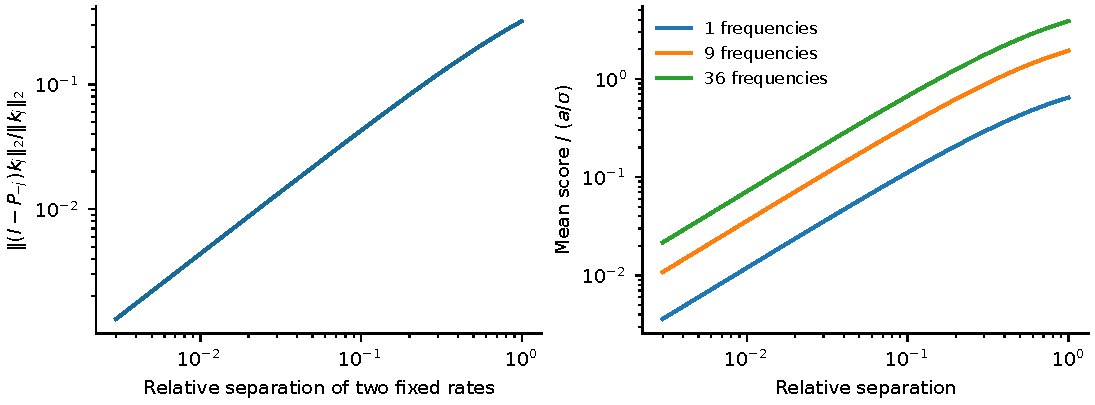
\includegraphics[width=\fulllength]{figures/geometry.pdf}
\caption{Fixed-design illustration of Equation~\eqref{eq:scoremean}, not a reconstruction benchmark. The two rates are $D/D_0=1$ and $1+\Delta$, with 32 equally spaced $bD_0$ values from 0 to 2.2. Left: the residualized-kernel norm decreases near collision. Right: coherent independent frequencies increase the expected standardized score by $\sqrt m$ for equal amplitudes. The rates and groups are fixed in this calculation.}\label{fig:geometry}
\end{adjustwidth}
\end{figure}

The operational screen estimates rates from the fitting data and groups frequencies after a signal mask. Consequently Proposition~\ref{prop:screen}'s calibration assumptions do not apply to the full estimator. We use $\alpha=0.01$ as a frozen screening parameter, not as a claimed family-wise error rate or chemical confidence level. If $\|v_j\|_2<10^{-10}\|k_j\|_2$, the implementation retains that component's allowed support: numerical nonidentifiability is not evidence of absence. Otherwise an entire group is allowed only when $Z_{jG}$ exceeds the threshold. NNLS still estimates separate nonnegative amplitudes at every retained frequency within an allowed group.

\subsection{Predictive comparison and automatic order}\label{sec:selection}
The available reconstruction rows are divided into an internal fitting set $T$ and an internal validation set $V$. Candidate paths include orders $0,1,\ldots,4$. For each path state, both the unrestricted support and, when different, the screened support are refined on $T$. A component with no allowed frequency is removed before refinement. Let $\widehat Y_{c,V}$ denote a candidate's prediction on $V$, and put
\begin{equation}\label{eq:val}
 L_c=\|\widehat Y_{c,V}-Y_V\|_F^2/\sigma^2.
\end{equation}
For numerically eligible candidates, let $c_*$ minimize $L_c$. We retain the set
\begin{equation}\label{eq:selection}
 \mathcal E=\left\{c:L_c\leq L_{c_*}+
 2\|\widehat Y_{c,V}-\widehat Y_{c_*,V}\|_F/\sigma+10^{-10}\right\}.
\end{equation}
Within $\mathcal E$, selection is lexicographic: fewer surviving rates, then fewer allowed amplitudes, then lower validation loss. The selected fixed support is refitted on $T\cup V$. The zero-signal model is a legitimate candidate. The selected $r$ is therefore automatic within a declared finite search, without access to the true order. Attaining the cap is reported rather than interpreted as evidence that no additional rates exist.

\begin{Proposition}[Conditional paired prediction variance]\label{prop:paired}
Let $P,Q$ be fixed predictions independent of $E$, and $Y=M+E$ with iid $N(0,\sigma^2)$ errors. Then
\begin{align}
 \mathbb E\{(\|P-Y\|_F^2-\|Q-Y\|_F^2)/\sigma^2\}
 &= (\|P-M\|_F^2-\|Q-M\|_F^2)/\sigma^2,\label{eq:pairedbias}\\
 \operatorname{Var}\{(\|P-Y\|_F^2-\|Q-Y\|_F^2)/\sigma^2\}
 &=4\|P-Q\|_F^2/\sigma^2.\label{eq:pairedvar}
\end{align}
\end{Proposition}
\begin{proof}
Subtracting the losses cancels the quadratic error term. The random remainder is $-2\langle P-Q,E\rangle/\sigma^2$, a centered normal variable with the variance in Equation~\eqref{eq:pairedvar}.
\end{proof}

This identity motivates the one-standard-deviation allowance in Equation~\eqref{eq:selection}; it does not provide a simultaneous confidence set after choosing the best of many candidates. Moreover, the benchmark signal mask uses all outer training rows, some of which become internal validation rows. Conditional independence of predictions and internal validation noise is therefore not exact after masking. The internal rule is explicitly heuristic. The eight external test acquisitions remain unused in the mask, candidate fitting, and selection, preserving an independent predictive evaluation for this full procedure. A future inferential version would need independent masking or cross-fitting and selection-adjusted calibration; neither has been retroactively attributed to the frozen benchmark.

\begin{Algorithm}[Spectral-support selection]
Given observed $b,Y,\sigma$, retained frequencies and physical bounds:
\begin{enumerate}
\item Sort the distinct acquisition coordinates and reserve internal validation rows. Construct groups from frequency coordinates without crossing large gaps.
\item Generate the native RAI or DOME path on internal fitting rows for orders zero to four.
\item For each state, construct the unrestricted and screened supports. Refine each through NNLS variable projection on fitting rows; save failures and diagnostics.
\item Predict internal validation rows, select by Equation~\eqref{eq:selection}, and apply the stated complexity tie-break.
\item Refit on all supplied outer training rows. Return rates, amplitudes, support, candidate losses, numerical diagnostics, and the automatically selected order. Export a mass-conserving 256-bin map for display.
\end{enumerate}
\end{Algorithm}

\subsection{The roles of RAI, DOME, TRAIn-MF, and TRAIn}
RAI's component path uses deterministic multistart nonnegative variable projection, including residual-based births, and its original selector minimizes a known-noise BIC-type score
$\mathrm{RSS}/\sigma^2+r(p+1)\log(np)$. All amplitudes are counted, including zeros. This is a heuristic adaptation of regular-model information criteria \cite{schwarz}: zero amplitudes and coincident rates create singular parameterizations. Singular learning theory explains why regular-model parameter-count penalties need not retain their usual interpretation in such settings \cite{watanabe}; we use these scores as documented heuristics.

DOME uses variance-based split proposals, frequency-dependent residual contrasts, and pairwise moment exchanges, followed by exact-kernel refinement. For example, splitting a mass $A$ at $m$ into $pA$ at $m-(1-p)\Delta$ and $(1-p)A$ at $m+p\Delta$ preserves mass and first moment, with
\begin{equation}\label{eq:split}
 Y_{\mathrm{split}}(b)-Ae^{-bm}
 =\tfrac12 Ae^{-bm}b^2p(1-p)\Delta^2+O(\Delta^3).
\end{equation}
This gives a proposal direction; every candidate is judged using the exact exponential model. The native DOME score is $\mathrm{RSS}/\sigma^2+2d+2d(d+1)/\max(np-d-1,1)$, where $d$ counts numerically positive amplitudes plus rates. It is also heuristic. RAI-S and DOME-S replace these native final order decisions with the same support/prediction procedure, while retaining their different candidate paths. Agreement between their outputs is not two independent demonstrations of benefit. No ablation here establishes a specific advantage of DOME's moment mechanism.

The archived TRAIn-MF solves a different problem. The suffix MF in TRAIn-MF is used in the multifrequency sense of the historical \texttt{TRAIn\_DOSY\_MFV31} header. Its matrix factorization $Y\approx KSA$ shares diffusion profiles (columns of $S$) across chemical shifts while allowing different component spectra (rows of $A$). It remains multifrequency when $r=1$: multiple frequencies need not imply multiple components. This terminology preserves the source lineage without equating the later constrained solver with the original TRAIn iteration. With $\widetilde Y=Y/s_Y$, $s_Y=\|Y\|_F/\sqrt{np}$ for nonzero data, its objective is
\begin{equation}\label{eq:mf}
 F(S,A)=\frac{\|KSA-\widetilde Y\|_F^2}{2p}
 +\frac{\lambda_S}{2}\|LS\|_F^2
 +\frac{\lambda_A}{2p}\|A\|_F^2,
\end{equation}
subject to Equation~\eqref{eq:mfconstraints}. Here $L$ discretizes density curvature on the log-diffusion grid, including mass-to-density conversion and quadrature weights. The reference uses 256 masses and $\lambda_S=\lambda_A=10^{-8}$. Conditional $A$ updates are augmented MATLAB NNLS problems; conditional $S$ updates enforce simplex constraints, and reduced-profile refinement follows if stationarity is inadequate. Monotone accepted objective values, being bounded below, converge as scalar values. This observation alone does not establish convergence of the factors or global optimality; KKT checks remain necessary. Block-coordinate convergence results require additional hypotheses on the objective and subproblem solutions \cite{tseng}. We do not assert that citing such a result establishes those hypotheses for every step of the archived solver.

The automatic TRAIn-MF selector first counts noise-resolved singular directions, caps the factor search at four and at that count, and then uses paired held-out losses among numerically converged candidates. Its count describes resolved predictive factors, with the limitation in Proposition~\ref{prop:rank}. The TRAIn-MF is included here as an unchanged distributional reference on a previously saved example, not as a newly tested winner on the atomic test. The provenance of this TRAIn-MF research line is explicit: the original TRAIn of Xu and Zhang \cite{train} was extended to a shared multifrequency model by Arrabal-Campos in \texttt{TRAIn\_DOSY\_MFV31} \cite{mfv31}. The archived source identifies its author and embeds a TRAIn-derived component solver using $h=\eta^2$, a Gauss--Newton model, truncated conjugate gradients, and trust-radius updates based on actual versus predicted reduction. This is a direct algorithmic antecedent of the TRAIn-MF extension, not an attribution inferred merely from a generic trust-region call.

The later TRAIn-MF reference used here replaces that embedded iteration with the constrained updates and stationarity checks associated with Equation~\eqref{eq:mf}. Thus the benchmarked solver and historical Version 3.1 differ numerically, while the TRAIn-MF lineage and authorship remain acknowledged. The public repository preserves both files and their identities \cite{software}. RAI-S and DOME-S use separate proposal mechanisms and a common support selector; a generic trust-region step does not by itself make either method an implementation of the original TRAIn.

\section{Reproducible Computational Study}\label{sec:experiments}
\subsection{Data partitions and frozen decisions}
The primary study contains 24 development problems and 48 new test problems, generated with disjoint seed ranges beginning at 510000 and 810000. A separate training bank for a neural policy comparison begins at 610000. A problem is an entire noisy DOSY matrix, not an individual spectral pixel. The support configuration was frozen before test evaluation: maximum order four, screening parameter $0.01$, validation stride four, one paired standard-deviation allowance, and at most 350 nonlinear function evaluations per support refinement.

An initial development run preferred support size before order. A weak-species development case revealed fragmentation, so the frozen version prefers order first. Both development runs are preserved. There was no test-set sweep of the screening parameter. The present manuscript reaggregates saved outputs and redraws figures; it does not refit the selected models or tune them to the illustrated ground truth.

Each new problem has 32 acquisition coordinates and 1024 frequencies uniformly spanning 10 to 0 ppm. Throughout the simulations, $D_0=10^{-9}\,\mathrm{m^2\,s^{-1}}$ and fitted rates are restricted to $[0.1,15]D_0$. The acquisition design is
\begin{equation}\label{eq:design}
 b_i=10^9 B\left(\frac{i}{31}\right)^\eta\ \mathrm{s\,m^{-2}},
 \quad i=0,\ldots,31,
\end{equation}
with independent $B\sim U(1.3,2.7)$ and $\eta\sim U(1.5,2.4)$. The component diffusion coefficients are positive and jointly shared across all frequencies. Their amplitudes have correlated Gaussian spectral peaks, including an overlapping region near 7.73 ppm and other peaks with different mixture proportions. The exact generator is included with the evidence package.

Eight families contain six problems each: one, two, or three separated rates; a three-rate weak-component family; a close-rate family; proportional component spectra; noise-only controls; and broad distributions. The six problems per family use SNR 50, 100, and 200 twice each, with independently generated parameters and noise. For positive signals, the maximum unattenuated spectral intensity is normalized to one in the generator and $\sigma=1/\mathrm{SNR}$. Solvers receive observations in these units, not true component normalizations.

Nominal separated rates are $(0.65,2.3,7.1)D_0$, using the first one or two as appropriate, with independent log-rate perturbations of standard deviation 0.10. Close rates use $(0.8,1.05,5.5)D_0$ with log-rate perturbations of standard deviation 0.02. In the weak family the third spectrum is multiplied by 0.04 before overall normalization; this is a spectral-amplitude multiplier, not a guarantee of exactly 4\% total mixture mass. In the proportional family $A_{j\cdot}$ equals $1,0.7,0.45$ times the same spectrum. Broad controls replace each atom by a lognormal distribution with log-width 0.18, using 24-point Gauss--Hermite forward quadrature. The forward generator uses the lognormal on its full positive domain; its histogram reference is truncated and renormalized on the fitted interval for plotting and shape evaluation. These controls deliberately violate the fitted atomic model.

Every fourth acquisition, using zero-based indices $i\bmod4=3$, is reserved for external testing. The remaining 24 rows are available to the reconstruction. A signal mask thresholds the mean of the first six available low-$b$ rows at $4\sigma/\sqrt6$, followed by two one-dimensional dilation steps. Noise-only controls instead inspect the fixed window $4<\mathrm{ppm}<4.65$. All methods in a comparison receive the same mask. Conditional on that mask, external test noise remains independent. The reported errors assess retained frequencies, not undetected parts of a full spectrum; losses caused by masking are not chemical absence certificates.

Within the 24 reconstruction rows, zero-based sorted positions \texttt{2:-1:4} form the internal validation set (six rows), leaving 18 rows for candidate fitting. Groups are split where adjacent selected frequency spacings exceed 1.6 times their 25th percentile. This rule assumes a substantially regular original spectral grid. It is a segmentation convention, not a learned chemical grouping. The final selected model uses all 24 reconstruction rows.

\subsection{Evaluation, denominators, and uncertainty summaries}
The primary quantitative panel is the 36 signal-present atomic problems. Six null cases are reported separately because normalized shape and true spectral leakage have no physical denominator there. Six broad cases are misspecification controls. An additional 24-problem archived bank contains finite-width diffusion profiles with one to three generating components, including close and proportional scenarios. It is transfer evidence and is never pooled with the new atomic bank.

Rates are paired to ground truth by a minimum-cost one-to-one assignment in absolute log distance; pairs beyond $0.25$ are then rejected. ``Order and rates recovered'' requires the correct total order and an accepted pair for every true rate. The tolerance corresponds to an approximate multiplicative factor of $e^{0.25}$, and is not a chemical identification standard. On finite-width controls, matching an atomic rate to a distribution center does not imply recovery of the distribution or a literal atom.

For each accepted pair $(j,k)$, define an evaluator-only meaningful spectral set
$\mathcal S_k=\{\ell:A^{\mathrm{true}}_{k\ell}>0.001\max_h A^{\mathrm{true}}_{kh}\}$ within the supplied mask. The leakage fraction is
\begin{equation}\label{eq:leakage}
 \ell_{\mathrm{spec}}=
 \frac{\sum_{(j,k)\ \mathrm{paired}}\sum_{\ell\notin\mathcal S_k}\widehat A_{j\ell}}
 {\sum_{(j,k)\ \mathrm{paired}}\sum_\ell\widehat A_{j\ell}}.
\end{equation}
The implementation assigns zero when its denominator is zero; therefore unmatched estimated mass is always reported alongside it, as a fraction of all estimated mass. Missing true rates are exposed by the recovery count. The $0.1\%$ threshold is an evaluation convention and never a fitting cutoff. It is also distinct from the display threshold in the DOSY figures.

External clean prediction error is $\|\widehat Y_U-Y_U^0\|_F/(\sigma\sqrt{|U|p})$ on the eight unused acquisitions $U$. It measures estimation error without adding a fresh noise variance; observed noisy-test errors are retained in the machine-readable results. Shape loss is $W_1$ in natural-log diffusion, evaluated after exporting both measures to the common 256-cell mass grid, normalizing per positive frequency, and weighting frequencies by true mass only in the evaluator. A missing positive estimate receives the declared span penalty $\log150$; it is not described as an actual transport distance. Total estimated mass is saved separately.

We report problem-level averages with equal weight per problem. The primary table excludes the null cases; Appendix~\ref{app:legacy} retains the earlier 42-case convention, whose zero contributions dilute shape averages. Bootstrap intervals resample whole paired problems 10,000 times with seed 9925. They are descriptive pointwise intervals for this small heterogeneous simulation bank, not simultaneous tests or calibrated population coverage. Different spectral frequencies are not treated as independent experimental replicates.

\subsection{Neural policy comparison and numerical verification}
RAI-Net is the action-ranking policy of Section~\ref{sec:rainetmath}, acting on the adaptive distributional objective in Equation~\eqref{eq:raihaar}. It does not directly predict the number of species. Retraining used 80 DOSY problems split by whole problem into 64 training and 16 validation problems, producing 2921 recorded action examples. The policy has two hidden layers of 48 units with hyperbolic-tangent activations. Training lasted 400 epochs and used a transformed noise-standardized internal validation prediction-gain target. The selected checkpoint was epoch 400, so convergence of learning is not claimed. The classical objective and numerical acceptance checks remained in force.

The original and retrained policies were evaluated on the predefined first 24 new test problems and all 24 archived transfer problems. The new neural panel contains three problems per scenario: 18 signal-present atomic, three null, and three broad-distribution cases. These are smaller panels than the atomic study. The network results are an auxiliary comparison, not an additional order-recovery experiment or evidence for the atomic support rule.

Numerical verification covers NNLS agreement with an independent implementation, finite-difference checks of the variable-projection Jacobian, coherent weak-signal screening, acquisition partition boundaries, and amplitude-scaling/frequency-permutation behavior. A direct comparison with MATLAB R2026a Update 2 \texttt{lsqnonneg} used 100 amplitude columns; a full MATLAB interface call was also checked. Numerical logs and hashes accompany the frozen outputs. Pseudoinverse-based local rate precision, boundary hits, and a residual-based atomic-model warning are exported as diagnostics; none is interpreted as a selection-adjusted confidence interval or goodness-of-fit test.

OpenAI Codex (GPT-6) assisted in manuscript drafting, algebraic derivations, code inspection, numerical reaggregation, figure-preparation code, reference checking, and compilation. Figure generation here uses deterministic scientific plotting of saved arrays; no generative image model supplies scientific data. Earlier benchmark computations are identified by their dated source archives. Human author review of all mathematical statements, numerical claims, and bibliographic records remains necessary before submission.

\section{Results}\label{sec:results}
\subsection{Atomic recovery and spectral leakage}
Table~\ref{tab:primary} reports the 36 signal-present atomic test problems. RAI-S reduces mean leakage from 5.166\% to 1.728\%, and DOME-S from 3.857\% to 1.728\%. The clean external prediction error decreases from 0.2870 to 0.2330 for RAI and from 0.2591 to 0.2330 for DOME. Binned shape loss decreases from 0.1523 to 0.1094 and from 0.1393 to 0.1094, respectively. These are paired changes on the same observations and masks.

\begin{table}[htbp]
\caption{New atomic test: 36 signal-present problems, excluding null and broad-distribution controls. Leakage and unmatched mass are percentages. $E_U$ is clean external RMSE divided by $\sigma$; $W_{1,h}$ is the binned log-diffusion shape score. A correct count is weaker than recovery of both order and rates.}\label{tab:primary}
\begin{adjustwidth}{-\extralength}{0cm}\centering\small
\begin{tabular}{lrrrrrr}\toprule
Method & Correct order & Order and rates & Leakage & Unmatched mass & $E_U$ & $W_{1,h}$\\\midrule
RAI & 17/36 & 17/36 & 5.166 & 6.774 & 0.2870 & 0.1523 \\
RAI-S & 25/36 & 23/36 & 1.728 & 7.257 & 0.2330 & 0.1094 \\
DOME & 26/36 & 22/36 & 3.857 & 7.019 & 0.2591 & 0.1393 \\
DOME-S & 25/36 & 23/36 & 1.728 & 7.257 & 0.2330 & 0.1094 \\
\bottomrule\end{tabular}

\end{adjustwidth}
\end{table}

The favorable averages do not hold for every endpoint. Unmatched estimated mass increases from 6.774\% to 7.257\% for RAI and from 7.019\% to 7.257\% for DOME. RAI's correct-order count rises from 17/36 to 25/36, but DOME's falls from 26/36 to 25/36. The stricter order-and-rates count improves from 17/36 to 23/36 and from 22/36 to 23/36. Thus the strongest common conclusion is improved spectral assignment and prediction, not uniformly improved component counting.

For RAI, the mean leakage change is $-3.438$ percentage points, with a descriptive 95\% paired bootstrap interval $[-5.282,-1.926]$. For DOME the change is $-2.129$ points, with interval $[-3.155,-1.268]$. The corresponding clean prediction changes are $-0.0540$ [$-0.0800,-0.0325$] and $-0.0261$ [$-0.0338,-0.0181$]. These intervals summarize the saved 36-case panel under the stated resampling convention; they do not adjust for multiple reported endpoints or establish external experimental performance.

RAI-S and DOME-S yield effectively identical primary summaries to the displayed precision. Their common post-proposal objective, support rule, and refinement can erase differences between proposal paths. These outcomes support the shared selection procedure and give no evidence that two independent improvements have been discovered.

\subsection{Scenario-level failures and a DOSY illustration}
Figure~\ref{fig:recovery} separates ordinary mixtures from difficult identification regimes. Both screened methods recover order and all rates in all six one-, two-, and three-separated-component cases. In close-rate cases they recover the correct order in 5/6 problems, but all rates in only 4/6. For proportional spectra they recover neither the full three-rate structure nor the correct order in any of six cases. The original DOME recovers the correct order in one of these cases, so the screened version has a visible regression.

In the weak family, the correct order is selected in 2/6 cases, but the weakest rate is matched in only 1/6; neither original method matches it in these six cases. In the one matched screened case, approximately 72\% of the true minority spectral mass lies within the retained allowed support. The support metric is a recall of permitted frequencies, not a claim of unbiased amplitude recovery. These results leave weak-species detection unresolved.

\begin{figure}[htbp]\centering
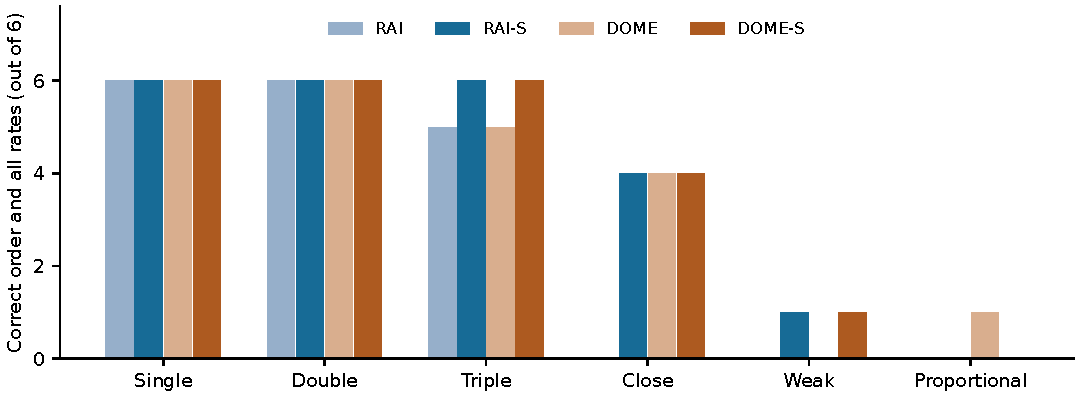
\includegraphics[width=\linewidth]{figures/recovery.pdf}
\caption{Recovery of both order and all rates by scenario in the new atomic test. Every bar has six independently generated problems. Matching uses a log-rate tolerance of 0.25. Narrow output bands and correct order alone do not imply successful localization.}\label{fig:recovery}
\end{figure}

\begin{figure}[p]
\begin{adjustwidth}{-\extralength}{0cm}\centering
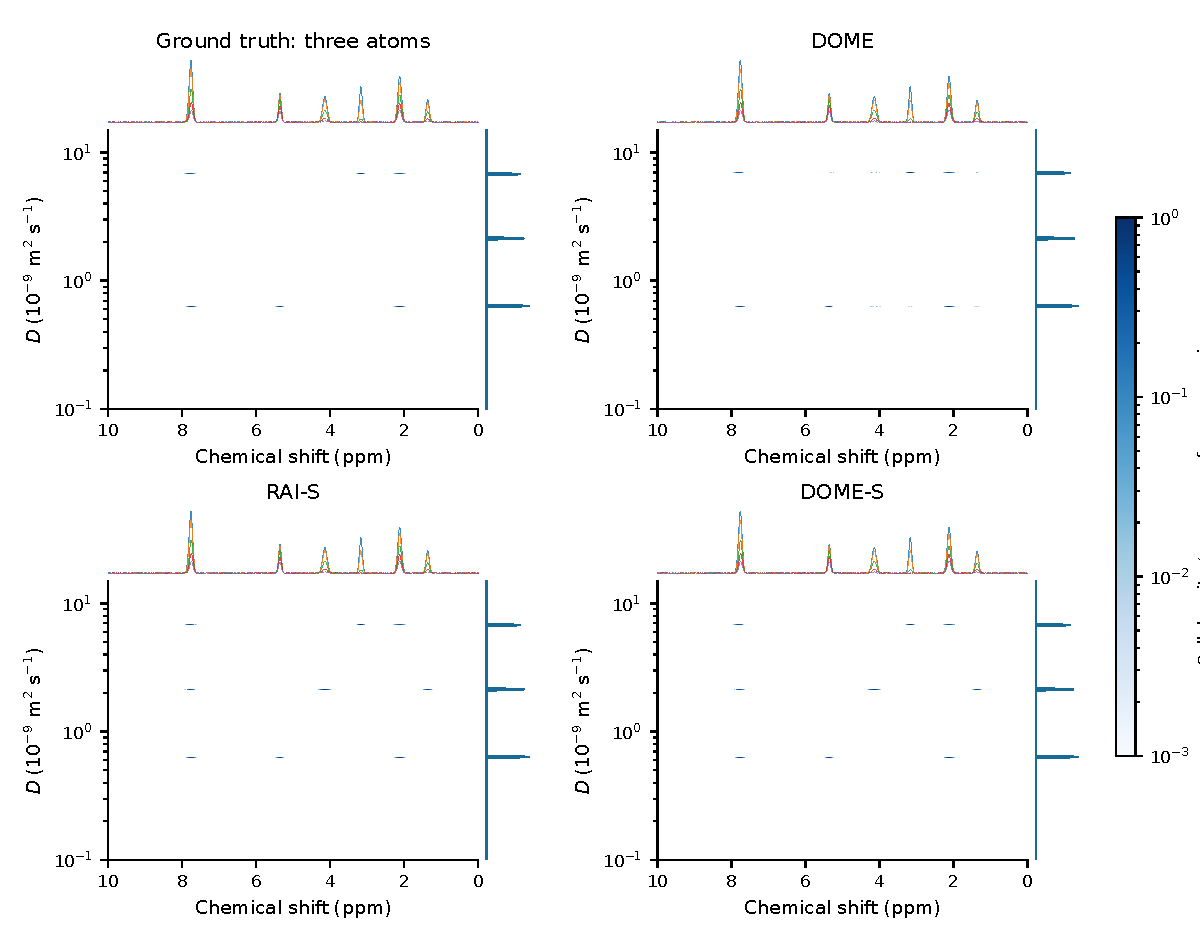
\includegraphics[width=\fulllength,height=.77\textheight,keepaspectratio]{figures/dosy_discrete.pdf}
\caption{Saved independent test problem 18, with three true atomic rates and SNR 200. The complete reference is shown alongside DOME and the two support-selected outputs. All panels use the same selected frequencies, 256-bin mass-to-density display, and common absolute reference maximum; values below 0.1\% of that maximum are not colored. The top traces show measured attenuation spectra. Side projections have separate horizontal scales. The display creates finite-width cells for atoms; it is not a recovered continuous width. Quantitative results use the unthresholded saved outputs.}\label{fig:dosyatomic}
\end{adjustwidth}
\end{figure}

Figure~\ref{fig:dosyatomic} provides one fixed illustration, rather than selecting a new representative after ranking the test outputs. The ground truth is displayed explicitly. Correlation is used through common rates and component-specific spectral amplitudes; it is not an assumption that every frequency has the same decay. The color threshold is a plotting convention applied to every panel and has no role in model order or support estimation.

\subsection{Null controls, broad distributions, and transfer}
All four atomic methods select the null model in all six noise-only controls. This observed count is not a guarantee of a population false-positive rate. On the six broad controls, the screened methods have clean prediction error 0.2382, compared with 0.3664 for RAI and 0.2837 for DOME. Their binned shape score is 0.1638, compared with 0.2686 and 0.1972. An atom model nevertheless cannot reproduce nonzero distributional width exactly. Counting its fitted rates against the number of generating broad profiles is a descriptive center-count comparison, not a valid literal atom-recovery claim.

On the 24 archived finite-width problems, leakage decreases from 1.245\% to 0.082\% for both native paths. Clean prediction error changes from 0.2650 to 0.2329 for RAI and from 0.2492 to 0.2329 for DOME. The selected-order count agrees with the number of generating profiles in 19/24 screened fits versus 18/24 native fits, while the stricter matching count remains 18/24. Transfer performance is encouraging for spectral assignment, but the differing true measure class prevents pooling it with the atomic test.

\begin{figure}[p]
\begin{adjustwidth}{-\extralength}{0cm}\centering
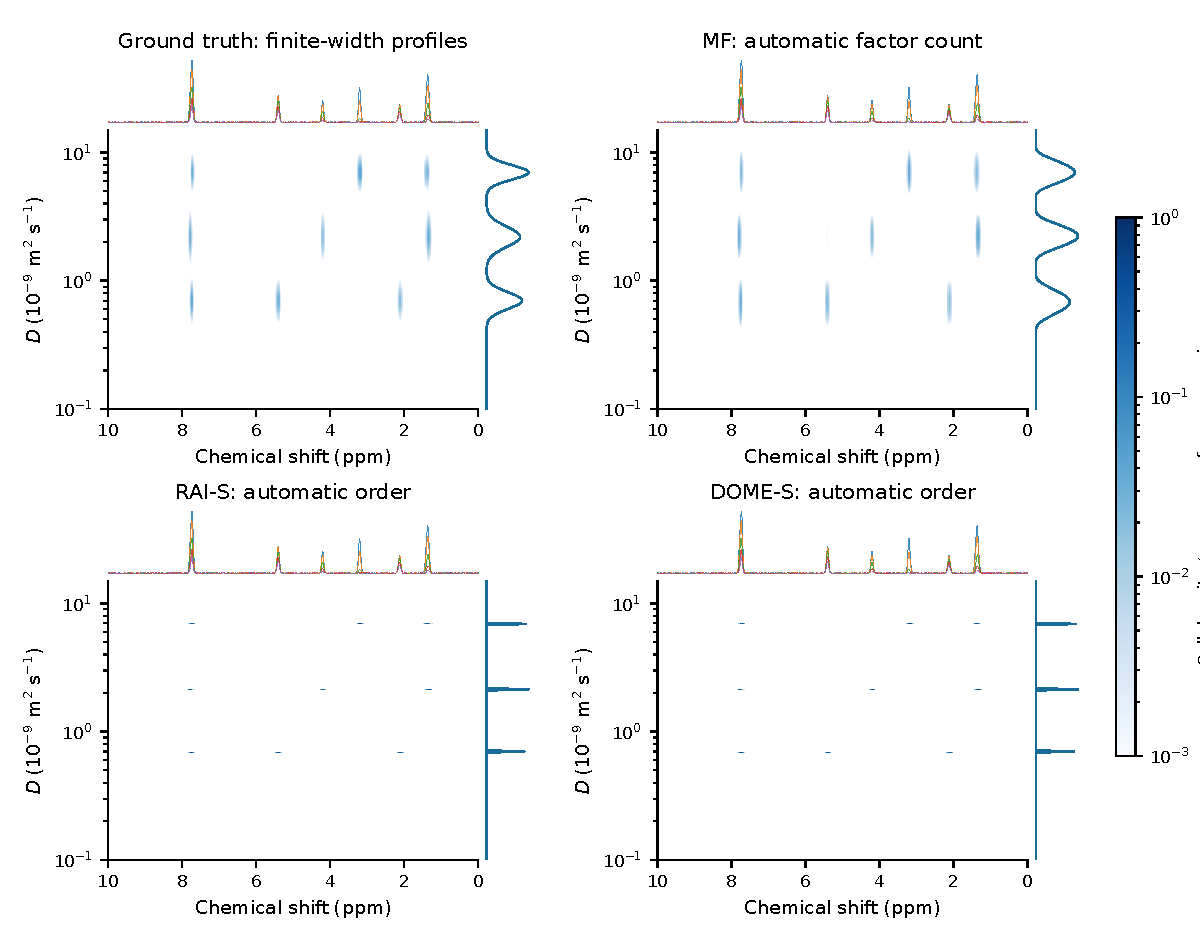
\includegraphics[width=\fulllength,height=.77\textheight,keepaspectratio]{figures/dosy_continuous.pdf}
\caption{Archived problem \texttt{r3\_snr200\_rep1}: three finite-width lognormal diffusion profiles, SNR 200, and 120 selected frequencies of 1024. Ground truth, the unchanged automatic MF reference, RAI-S, and DOME-S are shown. MF uses its original masses and original cell edges without remapping. Its factor count and the atomic methods' order are selected automatically but have different meanings. The common reference maximum is 63.34986357 in the saved cell-density units, with a 0.1\% display floor. Side projections are separately scaled. Fitted atoms occupy individual export cells and do not estimate the true widths.}\label{fig:dosycontinuous}
\end{adjustwidth}
\end{figure}

Figure~\ref{fig:dosycontinuous} retains the existing MF reconstruction and its native grid. For this case, the native atomic leakage of approximately 1.975\% decreases to 0.279\% after support selection, with three selected rates. The MF result is used to display the distinction between distributional factorization and atomic inference. It was not recomputed for this manuscript, and the figure is not a new all-method performance ranking. No conclusion about polymer molecular weights is drawn without a separate calibration and experimental analysis.

\subsection{Neural policy ablation}
Table~\ref{tab:net} reports the policy comparison. On 24 new test problems the relative change in mean binned shape score is approximately 0.041\%, with mean paired difference $-0.000111$ and bootstrap interval $[-0.001356,0.001105]$. The clean-error interval also includes zero. On the archived transfer panel, the shape score improves by approximately 1.48\%, but this does not establish an advantage on the new test. One fit per policy in the archived panel fails its numerical convergence criterion; both outputs remain in the reported averages.

\begin{table}[htbp]\centering
\caption{RAI-Net policy ablation on its predefined panels. These are distributional methods, so no chemical order-recovery count is assigned. All saved outcomes, including the two numerical failures, enter the averages.}\label{tab:net}
\begin{tabular}{llrrr}\toprule
Panel & Policy & $W_{1,h}$ & $E_U$ & Numerical success\\\midrule
New test, $n=24$ & Original & 0.272268 & 0.307991 & 24/24\\
 & Retrained & 0.272157 & 0.307921 & 24/24\\
Archived, $n=24$ & Original & 0.204769 & 0.326401 & 23/24\\
 & Retrained & 0.201739 & 0.326324 & 23/24\\\bottomrule
\end{tabular}
\end{table}

The new neural panel includes atomic, broad, and null cases, with zero shape-score contributions for nulls under the archived bookkeeping convention. Its averages therefore do not share the population of Table~\ref{tab:primary}. The policy ranks adaptive actions within an existing numerical procedure. It neither adds observations nor certifies the chemical support. These data do not support promoting the retrained policy as a superior substitute for the support-selected atomic estimator, and the two are not compared as if they shared the same output class.

\subsection{Numerical and provenance checks}
The archived audit verifies 144 support-selected fits across the new test and transfer banks. Their maximum relative amplitude KKT residual is $1.12\times10^{-15}$; the maximum normalized projected log-rate residual is $1.34\times10^{-7}$. Four poor-precision flags and four atomic-model-mismatch flags remain visible. The 100-column MATLAB NNLS comparison has relative prediction discrepancy $4.62\times10^{-17}$. Five targeted numerical tests pass. These figures are compatibility and numerical checks, not confidence bounds for chemical recovery.

An earlier clean extraction of the reproducibility bundle reproduced a selected prediction exactly. A later correction restored the original MF plotting grid and color floor without changing its numerical result or the support-selection core. The current manuscript hashes its input files and regenerates tables and figures from saved outputs. The MF array hash remains unchanged. Appendix~\ref{app:repro} specifies the replay and refitting scopes of the public release and the exploratory work retained in earlier archives.

\FloatBarrier
\section{Discussion}
The positive-measure formulation makes several distinctions operational. A discretization defines how mass is represented; regularization defines which admissible reconstructions are preferred; optimization determines how accurately a chosen criterion is solved; and identification concerns what the data support about the generating system. Their diagnostics differ. Increasing a display grid to 256 bins can reduce quantization error without providing 256 independent diffusion degrees of freedom. Reducing a residual can improve prediction while worsening distributional shape or changing the apparent number of species.

The support selector addresses a narrower failure: diffuse low-amplitude assignment of a shared atomic rate across unrelated frequencies. Residualization asks whether a proposed rate contributes beyond the other candidate decays, and aggregation can retain weak but coherent evidence. The unrestricted candidate remains available, so a hard screen is not imposed regardless of its predictive consequences. Automatic order is chosen from observations, with a null model and an explicit cap. Neither the true synthetic order nor a visually preferred component height enters selection.

There are important limits to this construction. The groups are geometric frequency windows, not chemical resonances obtained from a validated deconvolution. Screening a whole window assumes aggregate positive evidence; an overly large window can dilute a localized signal. Estimated nuisance rates can leave systematic residuals, and the screen does not account for model uncertainty. At near collision, residualization becomes poorly conditioned. Retaining support in that case avoids interpreting numerical collapse as absence, but cannot supply the missing information.

The prediction allowance is also a decision rule rather than a confidence procedure. Proposition~\ref{prop:paired} concerns a fixed pair of predictions independent of validation noise. Choosing the best candidate, reusing data in the mask, and searching multiple supports invalidate a direct inferential reading of one standard deviation. Reporting an independent external test protects the empirical comparison from that particular reuse, but does not calibrate the selected order. Independent mask construction, nested resampling, uncertainty over supports, and tests under correlated or estimated noise are reasonable subsequent studies, not properties established here.

The present evidence does not isolate every mechanism. Native-to-S comparisons change support restriction and final order selection together. Native baselines fit the 24 outer training rows directly, whereas the S procedure uses 18 rows for candidate construction followed by a 24-row refit. Both receive the same outer training information, but this is not a matched computation-budget ablation. A factorial comparison of screening only, predictive selection only, and the combined procedure would be required to apportion their effects. Since both native paths often reach the same final estimate, the study does not establish a special benefit of DOME's moment exchanges or RAI's particular starts. A global optimum is not certified, and a successful candidate search is not an exhaustive search over all continuous supports.

MF and atomic inversion answer different reconstruction questions. A positive factor profile can capture a broad polymer-like distribution, while a discrete model estimates a finite union of decay rates. Simplex normalization prevents the trivial scaling ambiguity but does not identify the factors chemically. The archived MF rank threshold counts resolved matrix directions; using that count as a cap can exclude weaker directions. This is particularly relevant when component spectra are nearly proportional. An improved automatic species selector cannot be obtained merely by relabeling a factor count.

The transfer illustration is useful because it reveals rather than hides this mismatch. RAI-S and DOME-S draw narrow bands for finite-width truth because their models are atomic. Their reduced spectral leakage is a benefit in a particular endpoint, not proof that the widths have been recovered. Similarly, lower binned transport loss for a policy within a limited domain does not demonstrate general neural superiority. The very small independent-test gain after RAI-Net retraining provides a concrete negative result.

The main empirical limitation is external validity. All new tests are synthetic, use known iid Gaussian noise, and operate after a signal mask. Baseline errors, phase errors, gradient calibration, relaxation contamination, exchange, convection, nonuniform spectral noise, and solvent suppression can violate this contract. No new experimental DOSY validation, molecular identity assignment, or molecular-weight calibration is included. The archived multi-method collection contains other implementations and adaptations, but its heterogeneous configurations are not substituted for a matched external comparator study here. Reproducibility of the current simulations and competence against strong independently tuned controls are different requirements.

\section{Conclusions}
Joint positive Laplace inversion benefits from keeping its mathematical objects explicit: masses, densities, atomic supports, and shared factors are not interchangeable. The derived results establish limited statements about discretization, uniqueness, and conditional selection statistics, while the implementation makes model order and spectral support data-dependent within a finite search. In the frozen atomic test, the shared support procedure reduces leakage and clean prediction error for both proposal paths, with modest improvement in full recovery and a small increase in unmatched mass. Proportional and weak mixtures remain difficult, and distributional controls expose the cost of an atomic assumption. These findings support an auditable selection framework and a bounded empirical improvement; they do not establish universal component identification.

\section*{Supplementary Materials}
Editable LaTeX, the four scientific figures, the per-problem frozen metrics, minimal synthetic figure inputs, source hashes, and replay scripts are provided in the public TRAIn-DOSY repository \cite{software}. The release also includes the historical TRAIn-MF Version 3.1, the native MATLAB reference, Python RAI-S/DOME-S, a local REST API, a C\# client, bilingual documentation, and three synthetic examples with separate ground truth. No public archival DOI has been assigned.

\section*{Author Contributions}
\draftfield{The following proposal based on author order must be confirmed by all three authors.}

Conceptualization, I.F. and F.M.A.-C.; methodology, V.V., I.F. and F.M.A.-C.; software, V.V. and F.M.A.-C.; validation, V.V., I.F. and F.M.A.-C.; formal analysis, V.V. and F.M.A.-C.; investigation and data curation, V.V.; writing---original draft preparation, V.V. and F.M.A.-C.; writing---review and editing, V.V., I.F. and F.M.A.-C.; visualization, V.V. and F.M.A.-C.; supervision, I.F. and F.M.A.-C.; project administration, F.M.A.-C. Funding acquisition remains unassigned.

\section*{Funding}
This research has been funded by the State Research Agency of the Spanish Ministry of Science and Innovation (PID2021-126445OB-I00), and by the Gobierno de Espa\~na MCIN/AEI/10.13039/501100011033 and Uni\'on Europea ``Next Generation EU''/PRTR (PDC2021-121248-I00, PLEC2021-007774 and CPP2022-009967).

\section*{Institutional Review Board Statement}
Not applicable to the computational synthetic experiments reported in this manuscript.

\section*{Informed Consent Statement}
Not applicable to the computational synthetic experiments reported in this manuscript.

\section*{Data Availability Statement}
Code and the synthetic materials described above are publicly available at \url{https://github.com/fmarrabal/train-dosy}, numerical software release \texttt{v0.1.0} \cite{software}. The method-specific formulations, structured Algorithm~\ref{alg:support}, expanded bibliography, and current manuscript are archived separately at \url{https://github.com/fmarrabal/train-dosy/releases/tag/manuscript-v6}; this documentation revision does not change the numerical cores or frozen results. The repository can regenerate the primary atomic benchmark and replay the manuscript figures and tables from saved arrays without re-estimation. The TRAIn-MF implementation requires a separately licensed MATLAB installation with Optimization Toolbox; its saved illustrative result is also supplied. The C\# interface invokes the reference API and is not an independent numerical implementation. The curated release retains the reported frozen exploratory neural metrics, but does not package end-to-end neural retraining or the entire historical algorithm survey. Earlier local archives and their identities are retained for provenance.

\section*{Conflicts of Interest}
\draftfield{A conflict-of-interest declaration must be provided by each author; it cannot be inferred from author order or the funding statement.}\par

\appendixtitles{yes}
\appendixstart
\appendix
\renewcommand{\theHequation}{appendix.\arabic{equation}}
\renewcommand{\theHproposition}{appendix.\arabic{proposition}}
\section{Further Mathematical and Numerical Details}
\subsection{Scaling and invariance}
In the atomic model, replacing $(Y,\sigma)$ by $(cY,c\sigma)$ for $c>0$ maps $A$ to $cA$, leaves rates fixed, and preserves the normalized objective and screening scores. The same transformation preserves the paired allowance in Equation~\eqref{eq:selection}. Thus, for unchanged candidate paths and masks, the exact-arithmetic decision is invariant to signal units. Finite solver tolerances and tie handling can introduce small numerical differences. Changing physical diffusion units with the reciprocal change in $b$ also preserves $bD$ and the predictions. Rescaling observations without rescaling $\sigma$ changes the statistical problem.

The TRAIn-MF objective has a related property through $\widetilde Y=Y/s_Y$: multiplying the data by $c$ changes $s_Y$ by $c$, leaves normalized factors unchanged, and rescales the exported amplitudes. Changing the number of frequencies is different. Averaging the data term by $p$ and the amplitude penalty by $p$ does not make arbitrary deletion of frequencies innocuous; the available shared information changes. The exact grid, quadrature, and regularization operator must also be kept fixed when claiming numerical equality of two TRAIn-MF outputs.

\subsection{A local separation expansion}
For the split in Equation~\eqref{eq:split}, write $\delta_1=-(1-\pi)\Delta$, $\delta_2=\pi\Delta$. Taylor expansion of $e^{-b(m+\delta)}$ gives a first-order term proportional to $\pi\delta_1+(1-\pi)\delta_2=0$, and a second-order term proportional to $\pi\delta_1^2+(1-\pi)\delta_2^2=\pi(1-\pi)\Delta^2$. The bounded-interval remainder is $O(\Delta^3)$ for a fixed finite acquisition design. The derivative in $\Delta$ vanishes at collision; a variance parameter can expose a nonzero second-order direction. This changes search geometry, not the measured information. After NNLS and rate refinement, moment preservation of the proposal is not a constraint on the final estimate.

\subsection{Support geometry and precision warnings}
For an interior fixed active set, the first-order rate information after treating amplitudes as nuisance involves projected kernel derivatives, weighted by amplitudes across frequencies. Extra rows or differently weighted spectra can add information. In proportional spectra, repeated columns may reduce variance by replication, while preserving the same decay-mixture proportions. If all relevant projected derivatives vanish, local rate separation fails irrespective of the plotted bin count.

The software additionally records the condition of the full residual Jacobian and the diagonal of a pseudoinverse of its Gram matrix. Residual-dependent terms, singular directions, active-set changes, and model selection prevent interpreting this output as a calibrated Fisher-information confidence interval. In particular, a pseudoinverse can return finite entries even when some directions are unidentifiable. The separate condition warning must be retained. A small normalized projected gradient establishes neither small parameter error nor precise component identification.

\section{Earlier Aggregation Convention}\label{app:legacy}
The support-study report originally summarized 42 atomic problems, including six null cases whose leakage and shape-score contributions were set to zero by convention. Table~\ref{tab:legacy} reproduces that aggregation for traceability. The primary text instead uses the 36 signal-present cases and reports the six null outcomes separately. This is a change in presentation and denominator, with no changed reconstruction or omitted failed positive case.
\begin{table}[htbp]
\caption{Earlier 42-case convention, including six null controls. Columns are defined as in Table~\ref{tab:primary}. The zero-valued null shape contributions are bookkeeping conventions, not normalized Wasserstein distances.}\label{tab:legacy}
\begin{adjustwidth}{-\extralength}{0cm}\centering\small
\begin{tabular}{lrrrrrr}\toprule
Method & Correct order & Order and rates & Leakage & Unmatched mass & $E_U$ & $W_{1,h}$\\\midrule
RAI & 23/42 & 23/42 & 4.428 & 5.806 & 0.2460 & 0.1306 \\
RAI-S & 31/42 & 29/42 & 1.481 & 6.220 & 0.1997 & 0.0938 \\
DOME & 32/42 & 28/42 & 3.306 & 6.016 & 0.2221 & 0.1194 \\
DOME-S & 31/42 & 29/42 & 1.481 & 6.220 & 0.1997 & 0.0938 \\
\bottomrule\end{tabular}

\end{adjustwidth}
\end{table}

\section{Reproducibility and Source Reuse}\label{app:repro}
The source archive \texttt{dosy\_support\_v2\_20260925\_corrected.zip} has SHA-256
\begin{quote}\small\ttfamily\path{fb130729aa69d258869a103c13e32df0fbe2861f771fdeb51e5660372a6b6bff}\end{quote}
The frozen numerical selector \texttt{support.py} has SHA-256
\begin{quote}\small\ttfamily\path{c9fcf58eb8226cf177f9b08692382cf33a6a9de4954c8f6c8d988d818be86531}\end{quote}
The unchanged TRAIn-MF result used in Figure~\ref{fig:dosycontinuous} has SHA-256
\begin{quote}\small\ttfamily\path{0ce63ab29e7cfbffc867ec569a6540827b9e63da9a30d5a125ce26558c639ed3}\end{quote}
The retrained neural checkpoint has SHA-256
\begin{quote}\small\ttfamily\path{a31627e4234a8c9464b20cd88d6ae15fd904560a4ecbf3c5a0657e26085bb786}\end{quote}

The public repository \url{https://github.com/fmarrabal/train-dosy} provides \texttt{paper/scripts/prepare\_evidence.py}. From the repository root, running that script reads the minimal saved synthetic fixture set, regenerates the primary and legacy tables, and produces the four scientific figures. No solver is called. The file \texttt{paper/build.ps1} compiles the editable LaTeX. The public \texttt{benchmarks/run\_atomic.py} separately reruns the 48-problem atomic protocol with the frozen generator, mask convention, and four methods; it does not substitute the new API discovery mask for the historical benchmark mask. Dependency versions, direct MATLAB instructions, API schemas, and C\# examples are documented in the release.

Source hashes in \texttt{provenance/source\_hashes.json} identify the preserved TRAIn-MF Version 3.1, later TRAIn-MF reference, atomic numerical core, and synthetic generator. The software citation distinguishes original TRAIn authorship from the multifrequency extension \cite{train,mfv31,software}. MATLAB's proprietary \texttt{lsqnonneg} implementation is called from the installed product and is not redistributed. The scientific quantities in the frozen result files were not altered when preparing this release.

The earlier Mathematics continuous-profile draft supplied the measure notation, density Jacobian, normalized positive-basis construction, partial-sharing objective, and conditional uniqueness argument. The RAI component revision supplied the finite-rate variable-projection perspective and its singular-model caveats. DOME's design record supplied the interpretation of moment-based proposals. All were reviewed against the corresponding mathematical expressions and implementation, and reworded for the present scope. Old Gaussian compendia and partial-sharing result tables use different protocols and are not relabeled as results of the new selector. A file-level reuse map accompanies the manuscript.

The current benchmark primarily tests internal RAI/DOME variants. A wider archived screen of ILT configurations is not a substitute for matched, independently tuned external comparisons: its entries include parameter variants and local adaptations. Publication claims should remain tied to the explicitly reported panel. The earlier paper draft, solver archive, and underlying prior work remain locally preserved. This revision identifies the public code release; it does not claim journal submission, acceptance, or approval of a completed author list.

\section{Additional Method Specifications and Historical Comparators}\label{app:extensions}
\subsection{The density-RAI graph}\label{app:graphdetails}
For column $\ell$, let $a_\ell=\max_i|y_{i\ell}|$, $v_{i\ell}=y_{i\ell}/a_\ell$, and $s_{i\ell}=\sigma_{i\ell}/a_\ell$, with a positive numerical floor on $a_\ell$. For two columns meeting the SNR requirement, the inspected density implementation uses
\begin{equation}\label{eq:graphdistance}
 d_{\ell m}=\frac1n\sum_i
 \frac{(v_{i\ell}-v_{im})^2}
 {s_{i\ell}^2+s_{im}^2+v_{i\ell}^2\max_k s_{k\ell}^2+v_{im}^2\max_k s_{km}^2}.
\end{equation}
An edge is admitted only below the fixed distance threshold and when both columns include the other among their nearest eligible neighbors; ties at the neighbor cutoff are retained. Then $W_{\ell m}=e^{-d_{\ell m}}$. The denominator accounts heuristically for uncertainty in shape normalization, but Equation~\eqref{eq:graphdistance} is not a calibrated test statistic. Estimating this graph from the available fitting rows changes the estimator; fixed-graph convexity applies conditionally after that construction.

\subsection{A feasible primal--dual gap for adaptive Haar RAI}\label{app:haargap}
Use the notation of Equation~\eqref{eq:raiadmm}, and let $\mathcal P(Z)=\lambda\sqrt p\sum_{h\geq2}\|Z_{h,:}\|_2$. Choose $N\leq0$ entrywise and a matrix $D$ with first row zero and $\|D_{h,:}\|_2\leq\lambda\sqrt p$ for detail rows. These are dual-feasible for the nonnegative cone and Haar penalty, respectively.
Let $u_\ell^*=H_\ell^{-1}(c_\ell-N_\ell-Q^\top D_\ell)$. Then
\begin{equation}\label{eq:haargap}
 \mathcal G(U,N,D)=\frac12\sum_\ell\|U_\ell-u_\ell^*\|_{H_\ell}^2
 +\mathcal P(QU)-\langle D,QU\rangle-\langle N,U\rangle.
\end{equation}
For $U\geq0$, every term is nonnegative, and completing the quadratic square shows that $\mathcal G$ equals a primal value minus the corresponding feasible dual lower bound. It therefore bounds suboptimality on this fixed tree. In ADMM the code uses the feasible primal iterate $V$, projects $\rho d_V$ to the nonpositive orthant, and projects $\rho d_Z$ to the row balls above. For the separate penalty the balls become entrywise intervals $[-\lambda,\lambda]$. At $\lambda=0$, it uses $N=\min(-\nabla f(U),0)$ and $D=0$ after ridge NNLS. Floating-point gap values are floored at zero to remove negative roundoff; this is a numerical bound construction, not interval arithmetic.

For completeness, let $m_{j\ell}$ be the current mass in leaf $j$, $\bar k_j$ its unit-mass kernel, and $w_j$ its log width. At each frequency the nuisance matrix concatenates columns $m_{j\ell}\bar k_j$ and $(m_{j\ell}w_j/2)\partial_x k(x_j)$ for occupied leaves, divided by that frequency's noise. Occupied means $m_{j\ell}>\max(0.02\max_hm_{h\ell},\operatorname{median}_i\sigma_{i\ell})$. Its left singular vectors with singular value at least one form $U_{\rm vis}$. For a prospective split contrast $t_j=(\bar k_{j,L}-\bar k_{j,R})/2$, put
\begin{equation}\label{eq:haarscore}
 v_{j\ell}=(I-U_{\rm vis}U_{\rm vis}^\top)(t_j/\Sigma_\ell),\quad
 s_{j\ell}=\frac{\langle v_{j\ell},(Y-B_{\rm fine}C)_\ell/\Sigma_\ell\rangle^2}
 {\|v_{j\ell}\|_2^2},\quad I_{j\ell}=m_{j\ell}\|v_{j\ell}\|_2.
\end{equation}
The score is set to zero if the denominator is at most $10^{-24}$ or $I_{j\ell}<0.05$. A raw score $s^0_{j\ell}$ omits nuisance projection. Joint-detail proposals rank leaves by $\sum_\ell s_{j\ell}$, private-detail proposals by $\max_\ell s_{j\ell}$, position proposals by $\sum_\ell s^0_{j\ell}$, and occupied-region proposals by $w_j\max_\ell m_{j\ell}$. At most four leaves are split per action, subject to capacity. The sibling pair with the smallest difference in its regional mass vectors supplies a merge proposal. These are deterministic heuristics inside the finite tree search, not tests of chemical identity.

\subsection{The 14 RAI-Net action features}\label{app:netfeatures}
For an action affecting leaves $I$, current leaf count $m$, candidate count $m'$, and fine count $q$, the feature vector used in Equation~\eqref{eq:rainet}, in stored order, is
\begin{align}\label{eq:netfeatures}
 \phi_a=\big(&m/q,\ m'/q,\ \one_{\rm merge},\ \one_{\rm position\ or\ occupied},\nonumber\\
 &\log(1+\textstyle\sum_{j\in I,\ell}s_{j\ell}),\
 \log(1+\max_{j\in I,\ell}s_{j\ell}),\
 \log(1+\textstyle\sum_{j\in I,\ell}s^0_{j\ell}),\nonumber\\
 &\log(1+\max_{j\in I,\ell}I_{j\ell}),\
 \frac{\sum_{j\in I,\ell}m_{j\ell}}{\max(\sum_{j,\ell}m_{j\ell},10^{-300})},\
 \frac{|I|^{-1}\sum_{j\in I}w_j}{\sum_jw_j},\nonumber\\
 &\log(1+\lambda),\ \log(1+n_{\rm supplied}),\ \log(1+p),\ \log(1+F_{\rm current})\big).
\end{align}
The acquisition-count feature is the number of supplied reconstruction rows before the internal split, not an external-test count. The action scorer sees the state derived from fitting rows; validation is used separately to train the revised priority target and to select completed penalty paths. Networks and checkpoints are therefore tied to the feature semantics as well as their matrix dimensions.

\subsection{DOME support averaging}\label{app:domeaverage}
The historical averaging variant holds the rates selected by native DOME fixed. At each frequency it enumerates subsets $J$ of these rates, including the empty subset, and computes NNLS amplitudes $a^{J}_\ell$ and $c_{J\ell}=\mathrm{RSS}_{J\ell}/\sigma^2+6|J|$. The penalty counts the nominal subset size even if some fitted amplitudes are zero. With temperature $T=0.5$, it solves the finite entropy-regularized averaging problem
\begin{equation}\label{eq:domeaverage}
 \min_{w\geq0,\,\sum_Jw_J=1}\sum_Jw_Jc_{J\ell}+T\sum_Jw_J\log w_J,
 \quad w_{J\ell}=\frac{e^{-c_{J\ell}/T}}{\sum_Le^{-c_{L\ell}/T}},\quad
 \bar a_\ell=\sum_Jw_{J\ell}a^J_\ell.
\end{equation}
Soft weights can retain weak contributions; they are not posterior probabilities or confidence levels. The rate set is not re-estimated, and single-frequency inputs bypass this averaging. This construction is mathematically different from DOME-S, which screens allowed supports, refines rates for each candidate, and selects by reserved-acquisition prediction.

\subsection{RAI-FLEX: joint atomic and smooth profiles}\label{app:raiflex}
RAI-FLEX uses $r_a$ atoms and $r_c$ shared smooth profiles. Let $\varphi_h$ be 24 nonnegative, unit-integral cubic B-splines in log diffusion, $G$ their integrated Laplace matrix, and $L_2$ their second-derivative quadrature operator. The predicted matrix is $H(d,C)A$ with $H(d,C)=[K(d),GC]$. The objective is
\begin{equation}\label{eq:raiflex}
 \min_{d,\,C\geq0,\,\one^\top C=\one^\top,\,A\geq0}
 \tfrac12\|(H(d,C)A-Y)/\Sigma\|_F^2+\tfrac\lambda2\|L_2C\|_F^2,
 \quad \lambda=0.01.
\end{equation}
Rates satisfy the physical bounds. NNLS eliminates $A$ at every evaluation. Initial optimization uses log rates and columnwise $C=\operatorname{softmax}(Z)$ with bounded logits, followed by direct simplex refinement to reach boundary profiles that a softmax gradient can represent poorly. The profile gradient is
\begin{equation}\label{eq:flexgrad}
 G_C=G^\top((HA-Y)/\Sigma^2)A_c^\top+\lambda L_2^\top L_2C,
 \qquad G_{Z,j}=C_j\odot\{G_{C,j}-(C_j^\top G_{C,j})\one\}.
\end{equation}
Here $A_c$ denotes the continuous-profile rows. A small logit gradient alone need not imply a small simplex KKT residual. After L-BFGS-B, up to 40 refinement sweeps alternate convex simplex quadratic profile updates, bounded atomic log-rate updates, and NNLS amplitudes, recording a scaled KKT residual with threshold $10^{-6}$.

The archived comparison searches allocations $r_a+r_c=r$ for $r=1,\ldots,4$; the general software default has a larger cap. There is no zero-model candidate in this RAI-FLEX search. A local effective dimension projects profile/rate tangent directions away from active spectral-amplitude directions. If $T_\perp$ is this weighted tangent matrix and $P$ the tangent penalty Hessian, the count is
\begin{equation}\label{eq:flexdf}
 d_{\rm eff}=d_A+\tr\{(T_\perp^\top T_\perp+P)^+
                                      T_\perp^\top T_\perp\}.
\end{equation}
Here $d_A=\sum_\ell\rank(\diag(\Sigma_\ell^{-1})H_{J_\ell})$ for the active amplitude subsets $J_\ell$; density tangent contrasts use spline coefficients above $10^{-5}$. The pseudoinverse is numerically truncated. The selector minimizes $\mathrm{RSS}/\sigma^2+2d_{\rm eff}+2d_{\rm eff}(d_{\rm eff}+1)/\max(1,np-d_{\rm eff}-1)$ over finite attained scores. It records stationarity but does not exclude every nonstationary candidate from this native selection. The count ignores active-set selection and nonlinear curvature and is therefore heuristic. Competing allocations within two score units are marked as type-ambiguous. The method does not certify that a fitted atom is a discrete molecule or that a broad profile is a polymer; these remain representation choices.

\subsection{Partial-C: one shared profile and unrestricted private densities}\label{app:partialalgorithm}
The generalized partial-C comparator instantiates Equation~\eqref{eq:partial} with 24 unit-integral cubic B-splines, one shared profile $s$, $C=sa+V$, $a,V\geq0$, and $\one^\top s=1$. Its penalty operators approximate the first derivative of the total density and the $L^2$ norm of the private density: $L^\top L=Q$ and $F^\top F=G$ in Section~\ref{sec:sharing}. These are different from RAI-FLEX's second-derivative penalty on its shared profiles. It fixes $\lambda_s=0.01$ and $\lambda_p=10$.

For each proposed $s$, Equation~\eqref{eq:partialdesign} gives the joint conditional NNLS fit of $(a_\ell,v_\ell)$, including the private penalty. With these amplitudes profiled out, the envelope gradient is
\begin{equation}\label{eq:partialgradient}
 \nabla_s J=\{K^\top(KC-Y)/\sigma^2+\lambda_sL^\top LC\}a^\top/p.
\end{equation}
Two observation-derived starts are refined by simplex-constrained SLSQP, with at most 300 iterations, and the lowest attained objective is retained. Shared-profile and conditional-linear KKT residuals at most $10^{-5}$ define its stationarity diagnostic. Proposition~\ref{prop:partial} proves conditional uniqueness under its stated conditions; it does not prove uniqueness of $s$ or of a physical decomposition. Shared rank is fixed to one in this comparator, not automatically selected. Because $V$ can represent every positive basis density, a rank-one shared term places no rank-one restriction on the complete signal.

\subsection{CIRCE reconstruction adapters: positive quadratics and a feasible-set check}\label{app:circe}
The archived CIRCE comparison adapts the reconstruction objectives to the benchmark design. Its 256 normalized piecewise-linear hats give masses $C\geq0$, operator $K$, and density derivative $R$. Let $a_h$ be the unnormalized hat areas and $J_a=\diag(1/a_h)$. Normalize observed columns to $f_\ell=Y_\ell/\max(\|Y_\ell\|_2,\sqrt n\sigma)$ and form
\begin{equation}\label{eq:circegraph}
 W_{\ell m}=\frac{\exp(-\|f_\ell-f_m\|_2^2/0.1)}{q\max(1,p-1)}\ (\ell\ne m),
 \quad W_{\ell\ell}=0,\qquad L_g=\diag(W\one)-W.
\end{equation}
Version 1 minimizes the convex quadratic
\begin{equation}\label{eq:circeone}
 F_1(C)=\tfrac12\|(KC-Y)/\sigma\|_F^2
       +\tfrac{0.02}{2}\|RC\|_F^2
       +\tfrac{0.01}{2}\tr(J_a^2 C L_g C^\top),\qquad C\geq0.
\end{equation}
Version 2 instead uses $C=TZ$, $Z\geq0$, where $T$ is a fixed positive mass-preserving decoder:
\begin{equation}\label{eq:circedecoder}
 T_{hk}=\frac{a_h\exp\{-(x_h-x_k)^2/(2w^2)\}}
 {\sum_j a_j\exp\{-(x_j-x_k)^2/(2w^2)\}},\qquad
 w=2\operatorname{mean}_h(x_{h+1}-x_h).
\end{equation}
With $s_\ell=\max(\max_i|Y_{i\ell}|,5\sigma)$, its objective is
\begin{equation}\label{eq:circetwo}
 F_2(Z)=\tfrac12\|(KTZ-Y)/\sigma\|_F^2
       +\tfrac{0.2}{2}\sum_\ell\frac{\|RTZ_\ell\|_2^2}{s_\ell^2}
       +\tfrac{0.01}{2}\tr(J_a^2TZL_gZ^\top T^\top).
\end{equation}
The decoder is part of the estimator, not display smoothing; its positive image is a restricted cone within the original basis representation. There is no learned decoder in this comparator. Both objectives have gradients given by the corresponding quadratic matrices, with $T^\top$ applied in Version 2. The usual implementation uses projected FISTA with restart and a fixed Hessian-norm Lipschitz bound. A ``strict'' configuration uses cyclic exact NNLS column blocks instead, including each graph column's off-diagonal contribution in the block right-hand side. Tolerances $10^{-6}$ and $10^{-10}$ distinguish numerical solves of the same objective, not additional physical inversion models.

The adapter then checks the returned physical masses against a residual cone and mass caps. Let $e_h$ bound each basis column's quadrature error uniformly across acquisitions, using 64 composite-trapezoid subdivisions per segment, and $\varepsilon=\sqrt{\chi^2_{np,0.95}}$. Its check is
\begin{equation}\label{eq:circecheck}
 \|(KC-Y)/\sigma\|_F+\sqrt n\|e^\top C\|_2/\sigma\leq\varepsilon,
 \qquad \one^\top C_\ell\leq
 \frac{[Y_{i_{\min},\ell}+\varepsilon\sigma]_+}{e^{-b_{\min}D_{\rm cap}}}.
\end{equation}
Here $i_{\min}$ is the smallest acquisition coordinate and $D_{\rm cap}$ is the comparator's supplied last diffusion-grid rate. Quadrature and mass checks include recorded floating-point tolerances; no interval-arithmetic certificate is asserted. The positive quadratic is solved first and checked afterwards. If its minimizer is feasible for the additional restrictions, it also minimizes the quadratic over that restricted set; otherwise the adapter reports an unverified estimate. It does not solve a constrained rescue problem. Its grid-center mass cap and data-dependent graph must not be promoted to universal continuous-measure coverage guarantees.

These adapters cover CIRCE reconstruction only. They do not compute CIRCE's alternative-measure bounds. The archived CIRCE-Net checkpoint was incompatible with this acquisition design, support, and basis, so no CIRCE-Net inference is claimed. Likewise, the full historical survey contains parameter configurations and design adaptations, not 60 independently validated mathematical inventions. None of these historical results is pooled into the primary support-selection panel.

\section{Conditional Uniqueness and Correlated-Noise Identities}\label{app:auditmath}
\subsection{What curvature regularization guarantees for a TRAIn-MF profile update}
The positive amplitude ridge in Equation~\eqref{eq:mfA} guarantees a unique conditional amplitude minimizer. The analogous claim for $S$ needs an additional condition: its curvature penalty is semidefinite, not positive definite.

\begin{Proposition}[Sufficient condition for a unique conditional profile update]\label{prop:mfprofile}
Fix $A$ and $\lambda_S>0$ in Equation~\eqref{eq:mf}. If the only matrix $U\in\R^{q\times r}$ satisfying
\begin{equation}\label{eq:mfprofileunique}
 KUA=0,\qquad LU=0,\qquad\one^\top U=0
\end{equation}
is $U=0$, the simplex-constrained $S$ subproblem has a unique minimizer.
\end{Proposition}
\begin{proof}
For a feasible affine direction $U$, the second directional derivative is
\begin{equation}\label{eq:mfsecondvariation}
 \frac{d^2}{dt^2}F(S+tU,A)=\|KUA\|_F^2/p+\lambda_S\|LU\|_F^2.
\end{equation}
The stated condition makes this positive for every nonzero direction with $\one^\top U=0$, so the objective is strictly convex on the simplex affine hull. The product of simplices is nonempty and compact, giving existence; strict convexity gives uniqueness. The condition is sufficient, not a necessary characterization of uniqueness at a boundary optimum.
\end{proof}

A degeneracy example shows why the condition matters. With two equal amplitude rows $A_{1,:}=A_{2,:}$, choose $v\ne0$ such that $Lv=0$ and $\one^\top v=0$, and set $U=[v,-v]$. Such a $v$ exists for the interior second-difference operator: $L$ has at most $q-2$ independent rows, and adding the single mass constraint still leaves a nontrivial null space. Then $UA=0$ and $LU=0$. At any strictly positive feasible $S$, sufficiently small $t$ preserves nonnegativity of $S+tU$, while both the prediction and the full objective remain exactly unchanged. Thus positive curvature regularization and simplex normalization can coexist with indistinguishable profile pairs. This is a counterexample to strict convexity of every conditional update, not a claim that the saved TRAIn-MF example has this degeneracy. It also explains why replacing a local KKT check by a statement of chemical uniqueness would be incorrect.

\subsection{Fixed-design scores under a specified covariance}\label{app:covariance}
The iid identities in Propositions~\ref{prop:screen} and \ref{prop:paired} have covariance-aware forms. These clarify their assumptions; the frozen solvers do not estimate or apply the covariance corrections below. Throughout this subsection $\operatorname{vec}$ stacks columns, and the covariance is specified independently of the evaluated observations.

\begin{Proposition}[Gaussian linear screening and paired quadratic loss]\label{prop:covariance}
Let $Y=M+E$, with $e=\operatorname{vec}E\sim N(0,\Omega)$. For fixed correct rates $M=KA$, a fixed frequency group $G$, its indicator $g_G\in\R^p$, and the residualized direction $v_j$ of Equation~\eqref{eq:score}, put $w=g_G\otimes v_j$. If $w^\top\Omega w>0$, then
\begin{equation}\label{eq:covscreen}
 \frac{w^\top\operatorname{vec}Y}{\sqrt{w^\top\Omega w}}
 \sim N\!\left(\frac{\|v_j\|_2^2\sum_{\ell\in G}A_{j\ell}}
                    {\sqrt{w^\top\Omega w}},1\right).
\end{equation}
For fixed predictions $P,Q$ independent of $E$, a fixed symmetric weight matrix $W\succeq0$, and $\delta=\operatorname{vec}(P-Q)$, let $L_W(P)=\|\operatorname{vec}(P-Y)\|_W^2$. Then
\begin{align}
 \mathbb E[L_W(P)-L_W(Q)]
 &=\|\operatorname{vec}(P-M)\|_W^2-\|\operatorname{vec}(Q-M)\|_W^2,\label{eq:covpairmean}\\
 \operatorname{Var}[L_W(P)-L_W(Q)]&=4\delta^\top W\Omega W\delta.\label{eq:covpairvar}
\end{align}
\end{Proposition}
\begin{proof}
The screening numerator is a fixed linear functional of a Gaussian vector. Its mean follows from $v_j^\top K_{-j}=0$ and $v_j^\top k_j=\|v_j\|_2^2$, and its variance is $w^\top\Omega w$. Expanding the two quadratic losses cancels $e^\top We$; the random remainder is $-2\delta^\top We$. Its mean is zero and its variance gives Equation~\eqref{eq:covpairvar}.
\end{proof}

If $\Omega=\sigma^2I$, Equation~\eqref{eq:covscreen} reduces to Equation~\eqref{eq:scoremean}; taking $W=\sigma^{-2}I$ also recovers Equation~\eqref{eq:pairedvar}. For separable covariance $\Omega=\Gamma\otimes\Sigma_b$, the screening variance factors as $(g_G^\top\Gamma g_G)(v_j^\top\Sigma_bv_j)$. The usual $\sqrt{|G|}$ signal gain therefore requires the independent-frequency variance scaling used in the benchmark. For positive-definite $\Omega$ and generalized least-squares weight $W=\Omega^{-1}$, the paired variance becomes $4\delta^\top\Omega^{-1}\delta$.

Estimated rates, groups, covariances, and the best prediction selected from the same data remain random. Substituting them into these formulas does not create a selection-adjusted test. In particular, holding out acquisition rows need not make errors independent when acquisition noise itself is correlated across those rows. A covariance model and a validation design respecting that dependence would be needed for a new calibrated procedure. No correlated-noise performance is inferred from the current iid benchmark.

\reftitle{References}
\begin{thebibliography}{99}
\bibitem{stejskal}
Stejskal, E.O.; Tanner, J.E. Spin Diffusion Measurements: Spin Echoes in the Presence of a Time-Dependent Field Gradient. \emph{J. Chem. Phys.} \textbf{1965}, \emph{42}, 288--292. \url{https://doi.org/10.1063/1.1695690}.

\bibitem{morris}
Morris, K.F.; Johnson, C.S., Jr. Diffusion-ordered two-dimensional nuclear magnetic resonance spectroscopy. \emph{J. Am. Chem. Soc.} \textbf{1992}, \emph{114}, 3139--3141. \url{https://doi.org/10.1021/ja00034a071}.

\bibitem{contin}
Provencher, S.W. CONTIN: A general purpose constrained regularization program for inverting noisy linear algebraic and integral equations. \emph{Comput. Phys. Commun.} \textbf{1982}, \emph{27}, 229--242. \url{https://doi.org/10.1016/0010-4655(82)90174-6}.

\bibitem{train}
Xu, K.; Zhang, S. Trust-Region Algorithm for the Inversion of Molecular Diffusion NMR Data. \emph{Anal. Chem.} \textbf{2014}, \emph{86}, 592--599. \url{https://doi.org/10.1021/ac402698h}.

\bibitem{itamed}
Urba\'nczyk, M.; Bernin, D.; Ko\'zmi\'nski, W.; Kazimierczuk, K. Iterative Thresholding Algorithm for Multiexponential Decay Applied to PGSE NMR Data. \emph{Anal. Chem.} \textbf{2013}, \emph{85}, 1828--1833. \url{https://doi.org/10.1021/ac3032004}.

\bibitem{palma}
Cherni, A.; Chouzenoux, E.; Delsuc, M.-A. PALMA, an improved algorithm for DOSY signal processing. \emph{Analyst} \textbf{2017}, \emph{142}, 772--779. \url{https://doi.org/10.1039/C6AN01902A}.

\bibitem{kaczmarz}
Gonz\'alez-L\'azaro, M.; Viciana, E.; Valdivieso, V.; Fern\'andez, I.; Arrabal-Campos, F.M. Regularized Kaczmarz Solvers for Robust Inverse Laplace Transforms. \emph{Mathematics} \textbf{2025}, \emph{13}, 2166. \url{https://doi.org/10.3390/math13132166}.

\bibitem{silt}
Yuan, B.; Ding, Y.; Kamal, G.M.; Shao, L.; Zhou, Z.; Jiang, B.; Sun, P.; Zhang, X.; Liu, M. Reconstructing diffusion ordered NMR spectroscopy by simultaneous inversion of Laplace transform. \emph{J. Magn. Reson.} \textbf{2017}, \emph{278}, 1--7. \url{https://doi.org/10.1016/j.jmr.2017.03.004}.

\bibitem{lin}
Lin, E.; Yang, Y.; Huang, Y.; Chen, Z. High-Resolution Reconstruction for Diffusion-Ordered NMR Spectroscopy. \emph{Anal. Chem.} \textbf{2020}, \emph{92}, 634--639. \url{https://doi.org/10.1021/acs.analchem.9b03865}.

\bibitem{arrabal2016}
Arrabal-Campos, F.M.; Oña-Burgos, P.; Fernández, I. Molecular weight prediction with no dependence on solvent viscosity. A quantitative pulse field gradient diffusion NMR approach. \emph{Polymer Chemistry} \textbf{2016}, \emph{7}, 4326--4329. \url{https://doi.org/10.1039/c6py00691d}.

\bibitem{arrabal2016correction}
Arrabal-Campos, F.M.; Oña-Burgos, P.; Fernández, I. Correction: Molecular weight prediction with no dependence on solvent viscosity. A quantitative pulse field gradient diffusion NMR approach. \emph{Polymer Chemistry} \textbf{2016}, \emph{7}, 5331. \url{https://doi.org/10.1039/c6py90124g}.

\bibitem{protein}
Arrabal-Campos, F.M.; Aguilera-Sáez, L.M.; Fernández, I. A diffusion NMR method for the prediction of the weight-average molecular weight of globular proteins in aqueous media of different viscosities. \emph{Analytical Methods} \textbf{2019}, \emph{11}, 142--147. \url{https://doi.org/10.1039/c8ay01817k}.

\bibitem{concentration}
Arrabal-Campos, F.M.; González-Lázaro, M.; Pérez, J.M.; Martínez Lao, J.A.; Fernández, I. Concentration-independent molecular weight determination of polymers via diffusion NMR: A universal approach across solvents. \emph{European Polymer Journal} \textbf{2025}, \emph{226}, 113710. \url{https://doi.org/10.1016/j.eurpolymj.2024.113710}.

\bibitem{photo2026}
Czarnota, M.; Cybularczyk-Cecotka, M.; Westermair, F.F.; Arrabal Campos, F.; Kapil, K.; Matyjaszewski, K.; Szczepaniak, G.; Urbańczyk, M. Real-time monitoring of photoinduced atom transfer radical polymerization by time-resolved diffusion NMR. \emph{Polymer Chemistry} \textbf{2026}, \emph{17}, 1109--1115. \url{https://doi.org/10.1039/d6py00103c}.

\bibitem{cyclic2021}
Ruiz Martínez, C.; Pérez, J.M.; Arrabal-Campos, F.M.; Batuecas, M.; Ortuño, M.A.; Fernández, I. Cyclic polylactide synthesis initiated by a lithium anthraquinoid: understanding the selectivity through DFT and diffusion NMR. \emph{Polymer Chemistry} \textbf{2021}, \emph{12}, 4083--4092. \url{https://doi.org/10.1039/d1py00547b}.

\bibitem{cyclic2023}
Ruiz Martínez, C.; Pérez, J.M.; Arrabal-Campos, F.M.; Rodríguez-Diéguez, A.; Choquesillo-Lazarte, D.; Martínez-Lao, J.A.; Ortuño, M.A.; Fernández, I. Lithium anthraquinoids as catalysts in the ROP of lactide and caprolactone into cyclic polymers. \emph{Polymer Chemistry} \textbf{2023}, \emph{14}, 452--461. \url{https://doi.org/10.1039/d2py01076c}.

\bibitem{chitosan2026}
Li, L.; Muguruza, A.R.; Arrabal-Campos, F.M.; Férnandez, T.; Fernández-García, S.; Muñoz-Flores, N.; Lorenzo, J.; Fernández, I.; Contreras-Caceres, R.; Guardia, P. Electrospun PVA-chitosan nanofibers with antibacterial properties for wound healing: unveiling the potential of low molecular weight chitosan. \emph{Journal of Materials Chemistry B} \textbf{2026}, \emph{14}, 9312--9326. \url{https://doi.org/10.1039/d6tb00497k}.

\bibitem{diffga}
Arrabal-Campos, F.M.; Álvarez, J.D.; García-Sancho, A.; Fernández, I. Molecular weight prediction in polystyrene blends. Unprecedented use of a genetic algorithm in pulse field gradient spin echo (PGSE) NMR. \emph{Soft Matter} \textbf{2017}, \emph{13}, 6620--6626. \url{https://doi.org/10.1039/c7sm01569k}.

\bibitem{dart}
Arrabal-Campos, F.M.; Aguilera-Sáez, L.M.; Fernández, I. Algebraic Reconstruction Technique for Diffusion NMR Experiments. Application to the Molecular Weight Prediction of Polymers. \emph{The Journal of Physical Chemistry A} \textbf{2019}, \emph{123}, 943--950. \url{https://doi.org/10.1021/acs.jpca.8b08584}.

\bibitem{mfv31}
Arrabal-Campos, F.M. \texttt{TRAIn\_DOSY\_MFV31}: Multi-Frequency/Multi-Component DOSY Inversion, Version 3.1. Source header dated January 2026; preserved in the TRAIn-DOSY software release 0.1.0 (2026). \url{https://github.com/fmarrabal/train-dosy/blob/v0.1.0/matlab/legacy/TRAIn_DOSY_MFV31.m}.

\bibitem{golub}
Golub, G.H.; Pereyra, V. The Differentiation of Pseudo-Inverses and Nonlinear Least Squares Problems Whose Variables Separate. \emph{SIAM J. Numer. Anal.} \textbf{1973}, \emph{10}, 413--432. \url{https://doi.org/10.1137/0710036}.

\bibitem{shearer}
Shearer, P.; Gilbert, A.C. A generalization of variable elimination for separable inverse problems beyond least squares. \emph{Inverse Probl.} \textbf{2013}, \emph{29}, 045003. \url{https://doi.org/10.1088/0266-5611/29/4/045003}.

\bibitem{lawson}
Lawson, C.L.; Hanson, R.J. \emph{Solving Least Squares Problems}; Classics in Applied Mathematics; SIAM: Philadelphia, PA, USA, 1995. Revised republication of the 1974 original. \url{https://doi.org/10.1137/1.9781611971217}.

\bibitem{denoyelle}
Denoyelle, Q.; Duval, V.; Peyr\'e, G.; Soubies, E. The sliding Frank--Wolfe algorithm and its application to super-resolution microscopy. \emph{Inverse Probl.} \textbf{2020}, \emph{36}, 014001. \url{https://doi.org/10.1088/1361-6420/ab2a29}.

\bibitem{discrete}
Provencher, S.W. A Fourier method for the analysis of exponential decay curves. \emph{Biophysical Journal} \textbf{1976}, \emph{16}, 27--41. \url{https://doi.org/10.1016/s0006-3495(76)85660-3}.

\bibitem{hansen}
Hansen, P.C. \emph{Rank-Deficient and Discrete Ill-Posed Problems}; SIAM: Philadelphia, PA, USA, 1998. \url{https://doi.org/10.1137/1.9780898719697}.

\bibitem{brd}
Butler, J.P.; Reeds, J.A.; Dawson, S.V. Estimating Solutions of First Kind Integral Equations with Nonnegative Constraints and Optimal Smoothing. \emph{SIAM Journal on Numerical Analysis} \textbf{1981}, \emph{18}, 381--397. \url{https://doi.org/10.1137/0718025}.

\bibitem{upen}
Borgia, G.C.; Brown, R.J.S.; Fantazzini, P. Uniform-Penalty Inversion of Multiexponential Decay Data. \emph{Journal of Magnetic Resonance} \textbf{1998}, \emph{132}, 65--77. \url{https://doi.org/10.1006/jmre.1998.1387}.

\bibitem{flint}
Teal, P.D.; Eccles, C. Adaptive truncation of matrix decompositions and efficient estimation of NMR relaxation distributions. \emph{Inverse Problems} \textbf{2015}, \emph{31}, 045010. \url{https://doi.org/10.1088/0266-5611/31/4/045010}.

\bibitem{fista}
Beck, A.; Teboulle, M. A Fast Iterative Shrinkage-Thresholding Algorithm for Linear Inverse Problems. \emph{SIAM Journal on Imaging Sciences} \textbf{2009}, \emph{2}, 183--202. \url{https://doi.org/10.1137/080716542}.

\bibitem{separable2d}
Venkataramanan, L.; Song, Y.-Q.; Hürlimann, M.D. Solving Fredholm integrals of the first kind with tensor product structure in 2 and 2.5 dimensions. \emph{IEEE Transactions on Signal Processing} \textbf{2002}, \emph{50}, 1017--1026. \url{https://doi.org/10.1109/78.995059}.

\bibitem{upen2d}
Bortolotti, V.; Brown, R.J.S.; Fantazzini, P.; Landi, G.; Zama, F. Uniform Penalty inversion of two-dimensional NMR relaxation data. \emph{Inverse Problems} \textbf{2017}, \emph{33}, 015003. \url{https://doi.org/10.1088/1361-6420/33/1/015003}.

\bibitem{mupen}
Bortolotti, V.; Landi, G.; Zama, F. Uniform Multipenalty Regularization for Linear Ill-Posed Inverse Problems. \emph{SIAM Journal on Scientific Computing} \textbf{2025}, \emph{47}, A790--A810. \url{https://doi.org/10.1137/23m1600943}.

\bibitem{mcr}
Tauler, R. Multivariate curve resolution applied to second order data. \emph{Chemometrics and Intelligent Laboratory Systems} \textbf{1995}, \emph{30}, 133--146. \url{https://doi.org/10.1016/0169-7439(95)00047-x}.

\bibitem{nmf}
Lee, D.D.; Seung, H.S. Learning the parts of objects by non-negative matrix factorization. \emph{Nature} \textbf{1999}, \emph{401}, 788--791. \url{https://doi.org/10.1038/44565}.

\bibitem{score}
Nilsson, M.; Morris, G.A. Speedy Component Resolution: An Improved Tool for Processing Diffusion-Ordered Spectroscopy Data. \emph{Analytical Chemistry} \textbf{2008}, \emph{80}, 3777--3782. \url{https://doi.org/10.1021/ac7025833}.

\bibitem{outscore}
Colbourne, A.A.; Meier, S.; Morris, G.A.; Nilsson, M. Unmixing the NMR spectra of similar species -- vive la différence. \emph{Chemical Communications} \textbf{2013}, \emph{49}, 10510--10512. \url{https://doi.org/10.1039/c3cc46228e}.

\bibitem{locodosy}
Colbourne, A.A.; Morris, G.A.; Nilsson, M. Local Covariance Order Diffusion-Ordered Spectroscopy: A Powerful Tool for Mixture Analysis. \emph{Journal of the American Chemical Society} \textbf{2011}, \emph{133}, 7640--7643. \url{https://doi.org/10.1021/ja2004895}.

\bibitem{gnat}
Castañar, L.; Dal Poggetto, G.; Colbourne, A.A.; Morris, G.A.; Nilsson, M. The GNAT: A new tool for processing NMR data. \emph{Magnetic Resonance in Chemistry} \textbf{2018}, \emph{56}, 546--558. \url{https://doi.org/10.1002/mrc.4717}.

\bibitem{espira}
Derevianko, N.; Plonka, G.; Petz, M. From ESPRIT to ESPIRA: estimation of signal parameters by iterative rational approximation. \emph{IMA Journal of Numerical Analysis} \textbf{2023}, \emph{43}, 789--827. \url{https://doi.org/10.1093/imanum/drab108}.

\bibitem{teicher}
Teicher, H. Identifiability of Finite Mixtures. \emph{The Annals of Mathematical Statistics} \textbf{1963}, \emph{34}, 1265--1269. \url{https://doi.org/10.1214/aoms/1177703862}.

\bibitem{drect}
Chen, B.; Wu, L.; Cui, X.; Lin, E.; Cao, S.; Zhan, H.; Huang, Y.; Yang, Y.; Chen, Z. High-Quality Reconstruction for Laplace NMR Based on Deep Learning. \emph{Analytical Chemistry} \textbf{2023}, \emph{95}, 11596--11602. \url{https://doi.org/10.1021/acs.analchem.3c00537}.

\bibitem{dream}
Chen, B.; Zhang, Y.; Wang, L.; Zhan, Z.; Guan, X.; Rong, Z.; Cui, Y.; Lin, E.; Cao, S.; Huang, Y.; Yang, Y.; Chen, Z. High-confidence reconstruction for Laplace inversion in NMR based on uncertainty-informed deep learning. \emph{Science Advances} \textbf{2025}, \emph{11}, eadw1379. \url{https://doi.org/10.1126/sciadv.adw1379}.

\bibitem{vallender}
Vallender, S.S. Calculation of the Wasserstein Distance Between Probability Distributions on the Line. \emph{Theory Probab. Appl.} \textbf{1974}, \emph{18}, 784--786. \url{https://doi.org/10.1137/1118101}.

\bibitem{schwarz}
Schwarz, G. Estimating the Dimension of a Model. \emph{Ann. Stat.} \textbf{1978}, \emph{6}, 461--464. \url{https://doi.org/10.1214/aos/1176344136}.

\bibitem{watanabe}
Watanabe, S. \emph{Algebraic Geometry and Statistical Learning Theory}; Cambridge University Press: Cambridge, UK, 2009. \url{https://doi.org/10.1017/cbo9780511800474}.

\bibitem{tseng}
Tseng, P. Convergence of a Block Coordinate Descent Method for Nondifferentiable Minimization. \emph{Journal of Optimization Theory and Applications} \textbf{2001}, \emph{109}, 475--494. \url{https://doi.org/10.1023/a:1017501703105}.

\bibitem{software}
Arrabal-Campos, F.M. TRAIn-DOSY: Positive Joint Laplace Inversion, Version 0.1.0; research software, 2026. \url{https://github.com/fmarrabal/train-dosy}.

\end{thebibliography}
\end{document}
